%\documentclass[a4paper,12pt,twoside]{report}
\documentclass[a4paper,12pt]{report}

%\usepackage{xeCJK}%汉字

%\usepackage[dvipsnames,table]{xcolor}%多颜色,颜色库要放在最前边,否则可能影响载入。
\usepackage[dvipsnames]{xcolor}%多颜色,颜色库要放在最前边,否则可能影响载入。

%\usepackage[options]{package-name}
%多个option不知道是不是用,隔开

%\usepackage[table]{xcolor}% to color the table

\usepackage{mdframed}%加灰色底框

\usepackage{empheq}%给文本加框

\usepackage[perpage]{footmisc}%footnote re-no. every page

%\usepackage{lipsum}

%\usepackage[utf8]{inputenc}
\usepackage{amsmath,amsthm,amssymb}%美国数学协会,proof 命令在这里。不是第一个
% 定义新的定理样式
\newtheoremstyle{mytheoremstyle}% 请替换为你喜欢的样式名
  {0.5em}% 上间距
  {0.5em}% 下间距
  {\itshape}% 定理内容的字体样式
  {}% 缩进量
  {\bfseries}% 定理标题的字体样式
  {  }% 标题后的标点符号
  {0.0em}% 标题与内容之间的距离
  {}% 定理头部的额外规范
\theoremstyle{mytheoremstyle}% 创建新的定理环境
\newtheorem{theorem}{Theorem}

\usepackage{float}%调整图片位置的包,才能用[H]
\usepackage{adjustbox}%供画图用
\definecolor{mycolor}{RGB}{82, 140, 164}%调好的蓝色,做边框
%E.G.一个画图例子
% begin{figure}[H] % [H] forces figure to be output where it is defined in code (it suppresses floating)
% 		\adjustbox{frame=1pt,frame,margin=0.5,color=mycolor}{\includegraphics[width=\linewidth]{pics/The Nectar login page.png}} % Figure image
% 		\caption{\small Regenerated boundary shape and surface charge density of the charged droplets as described by Crowdy (2015), with different value of capillarity effort coefficients applied.}
% 	\end{figure}


\usepackage{extarrows}%长等号,且上下可添加文字
%https://www.latexstudio.net/archives/8004.html
%$$ A\xlongequal[sub-script]{super-script}B $$


%链接:https://www.zhihu.com/question/617310608/answer/3166157888
%\usepackage{amssymb}%可以打\therefore 因为所以符号的命令

\usepackage{mathrsfs}%花体字母

\numberwithin{equation}{section}%和上一个,让公式按 section 编号

\usepackage{bm}
%\usepackage{natbib}

%%%%%%%%%%%%%%%%%%%%%%%%%%%%%%%%%%%%%%%%%%%%%%%%%%%%%%%%
%annotate eqn packages
\usepackage{tikz}
\usetikzlibrary{backgrounds}
\usetikzlibrary{arrows,shapes}
\usetikzlibrary{tikzmark}
\usetikzlibrary{calc}

\usepackage{mathtools}
\usepackage{hyperref}
\usepackage{cleveref}
\usepackage{annotate-equations}
%%%%%%%%%%%%%%%%%%%%%%%%%%%%%%%%%%%%%%%%%%%%%%%%%%%%%%%%%%%%%%%%%%%%%%%%%%%

%\usepackage{float}%禁止表格浮动,相应的命令是\FloatBarrier,但实际上似乎不管用,用[h!]解决的。


%\usepackage[a4paper,scale=0.8]{geometry}%格式

%\usepackage{color}


%\usepackage{lipsum}

\usepackage{ragged2e}%使用\justify 回到正常对齐

\usepackage{tabularray}

\usepackage{shadowtext}

%\usepackage[utf8]{inputenc}
\usepackage[T1]{fontenc}
\usepackage{lmodern}
\usepackage{amsfonts}
\usepackage{epstopdf}
%\usepackage{matlab}

\sloppy%不知道干嘛用,matlab的文件带的
\epstopdfsetup{outdir=./}
\graphicspath{ {./a1q3_images/} }

\usepackage{pdfpages}%嵌入pdf页面,用\includepdf[pages={1,2}]{1.pdf} %[pages={3},scale=0.5] 命令可用

%公式字母划去,用\cancel{}
\usepackage{cancel}
%\usepackage[thicklines]{cancel}

\usepackage{graphicx} % Required for inserting images


%以下三个是griffiths用的表示电磁学上场点和源点差的矢量的符号,需要相应的两个pdf的支持。
%\def\rcurs{{\mbox{$\resizebox{.16in}{.08in}{\includegraphics{ScriptR}}$}}}
%\def\brcurs{{\mbox{$\resizebox{.16in}{.08in}{\includegraphics{BoldR}}$}}}
%\def\hrcurs{{\mbox{$\hat \brcurs$}}}

%%%%%%%%%%%%%%%%%%%%%%%%%%%%%%%%%%%%%%%%%%%%%%%%%%%%%%%%%%%%%%%%%%%%%%%%%%
\usepackage{fancyhdr}
\pagestyle{fancy}
\usepackage{lastpage}

% Define Header
%\lhead{Yuan Liu (313350417)}
%\chead{Physics 335 QM formulas}
%\rhead{\today}

% Define Footer
%\lfoot{}
%\cfoot{Page \thepage \,of \pageref{LastPage}}
%\rfoot{}

%\fancyhead{} % 页眉清空
\renewcommand{\headrulewidth}{0pt} % 去页眉线
%Define width of horizontal line in the header
%\renewcommand{\headrulewidth}{0.4pt}
\renewcommand{\footrulewidth}{0.2pt}
\usepackage[numbers]{natbib}
%\bibliographystyle{plain}
%\citestyle{authoryear}
%在 LaTeX 中,如果你想要使用哈佛风格(Harvard style)的文中引用,并且不希望出现数字编号,你可以使用 natbib 宏包结合 authoryear 样式。这个组合可以让你在文中引用作者和年份,并且不出现数字编号。
\usepackage[perpage]{footmisc}%footnote re-no. every page
%\usepackage{perpage}
%%%%%%%%%%%%%%%%%%%%%%%%%%%%%%%%%%%%%%%%%%%%%%%%%%%%%%%%
%annotate eqn packages
\usepackage{tikz}
\usetikzlibrary{backgrounds}
\usetikzlibrary{arrows,shapes}
\usetikzlibrary{tikzmark}
\usetikzlibrary{calc}

\usepackage{mathtools}
\usepackage{hyperref}
\usepackage{cleveref}
\usepackage{annotate-equations}
%%%%%%%%%%%%%%%%%%%%%%%%%%%%%%%%%%%%%%%%%%%%%%%%%%%%%%%%%%%%%%%%%%%%%%%%%%%

\usepackage{extarrows}%长等号,且上下可添加文字
%https://www.latexstudio.net/archives/8004.html
%$$ A\xlongequal[sub-script]{super-script}B $$

\usepackage{datetime}
\settimeformat{ampmtime}%add am/pm. see https://texblog.org/2011/05/02/date-and-time/

\usepackage{fancyhdr}
%\pagestyle{fancy}
\fancyfoot[C]{\thepage} % 在页脚中间添加页码

\usepackage{lastpage}


\usepackage{float}%调整图片位置的包,才能用[H]
\usepackage{adjustbox}%供画图用
\definecolor{mycolor}{RGB}{82, 140, 164}%调好的蓝色,做边框
%E.G.一个画图例子
% begin{figure}[H] % [H] forces figure to be output where it is defined in code (it suppresses floating)
% 		\adjustbox{frame=1pt,frame,margin=0.5,color=mycolor}{\includegraphics[width=\linewidth]{pics/The Nectar login page.png}} % Figure image
% 		\caption{\small Regenerated boundary shape and surface charge density of the charged droplets as described by Crowdy (2015), with different value of capillarity effort coefficients applied.}
% 	\end{figure}

\usepackage{extarrows}%长等号,且上下可添加文字
%https://www.latexstudio.net/archives/8004.html
%$$ A\xlongequal[sub-script]{super-script}B $$

%链接:https://www.zhihu.com/question/617310608/answer/3166157888
%\usepackage{amssymb}%可以打\therefore 因为所以符号的命令

\usepackage{mathrsfs}%花体字母

\numberwithin{equation}{section}%和上一个,让公式按 section 编号

\usepackage{titlesec}
% 自定义 chapter 标题格式,设置顶部间距为 0,底部间距为 20pt
\titleformat{\chapter}[hang]{\huge\bfseries}{\thechapter}{1em}{}
\titlespacing*{\chapter}{0pt}{-10pt}{20pt}  % 调整章节标题的上方和下方间距

\usepackage{amsmath,amsthm,amssymb}%美国数学协会,proof 命令在这里。不是第一个
% 定义新的定理样式
%\newcommand{\apx}{\, \~{} \,}
\newcommand{\im}{\mathrm{i} \,}
\newcommand{\df}{\,\mathrm{d}}%定义命令来表示微分符号



\newtheorem{thm}{Theorem}[section]%
%\newtheorem{eg}{E.g.}[section]%
%\newtheorem{defn}{Definition}[section]%
\newtheorem{defn}[thm]{Definition}% def 不工作,需定义新命令 defn
\newtheorem{eg}[thm]{Example}%
%替换的两条,使 eg thm def 统一编号,便于查找。
\newtheorem{prop}[thm]{Propostion}%
\newtheorem{prf}[thm]{Proof}%


\def\Xint#1{\mathchoice
   {\XXint\displaystyle\textstyle{#1}}%
   {\XXint\textstyle\scriptstyle{#1}}%
   {\XXint\scriptstyle\scriptscriptstyle{#1}}%
   {\XXint\scriptscriptstyle\scriptscriptstyle{#1}}%
   \!\int}
\def\XXint#1#2#3{{\setbox0=\hbox{$#1{#2#3}{\int}$}
     \vcenter{\hbox{$#2#3$}}\kern-.5\wd0}}
\def\ddashint{\Xint=}
\def\dashint{\Xint-}
%\dashint gives a single-dashed integral sign, \ddashint a double-dashed one.
%https://texfaq.org/FAQ-prinvalint


\usepackage[left=2cm,right=2cm,top=2cm,bottom=3cm]{geometry}
%\geometry{a4} 
\usepackage[english]{babel}
\usepackage{fancyhdr}
\setlength{\headheight}{15pt} 
\usepackage{titlepic}
\usepackage{fancyhdr}
\usepackage{graphicx}
\usepackage{lipsum}
\usepackage{titling}
\usepackage{textcomp}
\usepackage{gensymb}
\usepackage{amsfonts}
\usepackage{multirow}
\usepackage{subcaption}
\usepackage{siunitx}
\usepackage{microtype}  % %minutely improves kerning
%\usepackage[active,floats]{preview}
% % % %Table of contents
\usepackage[intoc]{nomencl}
\usepackage{color}
\makeatletter
\if@titlepage
%\titlepic{
\includegraphics[width=0.30\textwidth]{C0/Figs/Imperial_College_London_crest}}
\renewcommand\maketitle{
    \begin{titlepage}%
    \begin{center}
        \let\footnotesize\small
        \let\footnoterule\relax
        \let \footnote \thanks
        \Large\sf Imperial College London \\
            %\linebreak
            Department of Mathematics
            \rm
            \vskip 2in
        %
            {\LARGE \sf\textbf{\@title} \par}%
            \vskip 3em% %% Change this space if you wish
            {\large
                \lineskip .75em%
                \begin{tabular}[t]{c}%
                \LARGE\sf\@author
                \\
                \LARGE\sf CID:01586955
                \\
                \LARGE\sf Supervisor: Dr. Samuel Brzezicki
                \end{tabular}\par%
        
            }%
         \@tpsepspace% %% uncomment if you need space.
%         \@titlepic

            \vskip 10em
            \vskip 7em%   %% Change this space if you wish
\iffalse   
          \sf Submitted in part fulfilment of the requirements
          \linebreak
          for the degree of Master of Applied Mathematics at
          \linebreak
\fi
          Master of Applied Mathematics
          \linebreak
          Imperial College London
          \linebreak
          \currenttime, \today
          \vfil
          \end{center}
    \end{titlepage}%
%    \setcounter{footnote}{0}%
%    \global\let\thanks\relax
%    \global\let\maketitle\relax
%    \global\let\@thanks\@empty
%    \global\let\@author\@empty
%    \global\let\@date\@empty
%    \global\let\@title\@empty
%    \global\let\@titlepic\@empty
%    \global\let\title\relax
%    \global\let\author\relax
%    \global\let\date\relax
%    \global\let\and\relax
%    \global\let\titlepic\relax
}
\fi
\makeatother
\makenomenclature
%\RequirePackage[intoc]{nomencl}
%\makenomenclature
%\renewcommand{\nomgroup}[1]{%
%\ifthenelse{\equal{#1}{A}}{\item[\textbf{Roman Symbols}]}{%
%\ifthenelse{\equal{#1}{G}}{\item[\textbf{Greek Symbols}]}{%
%\ifthenelse{\equal{#1}{Z}}{\item[\textbf{Acronyms / Abbreviations}]}{%
%\ifthenelse{\equal{#1}{R}}{\item[\textbf{Superscripts}]}{%
%\ifthenelse{\equal{#1}{S}}{\item[\textbf{Subscripts}]}{%
%\ifthenelse{\equal{#1}{X}}{\item[\textbf{Other Symbols}]}
%{}
%}% matches mathematical symbols > X
%}% matches Subscripts           > S
%}% matches Superscripts         > R
%}% matches Abbreviations        > Z
%}% matches Greek Symbols        > G
%}% matches Roman Symbols        > A
\def\abstract{
  \begin{center}{
    \large\bf Abstract}
  \end{center}
  \small
  %\def\baselinestretch{1.5}
  \linespread{1.5}
  \normalsize
}
\def\endabstract{
  \par
}

\newenvironment{acknowledgements}{
  \cleardoublepage
  \begin{center}{
    \large \bf Acknowledgements}
  \end{center}
  \small
  \linespread{1.5}
  \normalsize
}{\cleardoublepage}
\def\endacknowledgements{
  \par
}

\newenvironment{dedication}{
  \cleardoublepage
  \begin{center}{
    \large \bf Dedication}
  \end{center}
  \small
  \linespread{1.5}
  \normalsize
}{\cleardoublepage}
\def\enddedication{
  \par
}

%\includeonly{CA1/chapterA1}
\usepackage{keystroke}
\usepackage{xcolor}
\usepackage{listings}
\lstset{
  basicstyle=\ttfamily,  %basicstyle=\footnotesize,
  columns=fullflexible,
  showspaces=false,
  showtabs=false,
  breaklines=true,
  showstringspaces=false,
  breakatwhitespace=true,
  escapeinside={(*@}{@*)}
}
\usepackage{setspace}
\usepackage{amsmath}
\usepackage{mathtools}
\usepackage{upgreek}
\usepackage{units}
\usepackage{lscape}
\usepackage{pbox}
\usepackage[tableposition=top]{caption}
\usepackage{float}
\floatstyle{plaintop}
\restylefloat{table}
\usepackage[version=3]{mhchem}
%\usepackage[sectionbib]{chapterbib}
%\bibliographystyle{plain}
%\usepackage{bibentry}
%\usepackage{biblatex}
%\usepackage{navigator}
%\usepackage[hidelinks]{hyperref}
%\hypersetup{
%    colorlinks=false, %set true if you want colored links
%    linktoc=all,     %set to all if you want both sections and subsections linked
%    linkcolor=black,  %choose some color if you want links to stand out
%}
%
%\vspace*{6mm}}
%\title{Study of Static Electrowetting Droplets at Specific Contact Angles: Conformal Mapping, Complex Potentials, and Droplet Shapes}
\title{Study of Electrowetting at Specific Contact Angles: Mapping, Potentials, and Shapes}

\author{Yuan \textsc{Liu}}

\begin{document}
\onehalfspacing%better though, same as \linespread{1.5}   
\pagestyle{fancy}

\maketitle

%\pagenumbering{roman}
%\topskip20pt
\vspace*{\fill}
\begin{center}
I hereby declare that this thesis and the work reported herein was composed by and originated entirely from me. Information derived from the published and unpublished work of others has been acknowledged in the text and references are given in the list of sources.

\begin{flushright}
Samuel John Cooper (2015)
\end{flushright}
\end{center}
\vspace*{\fill}

The copyright of this thesis rests with the author and is made available under a Creative Commons Attribution Non-Commercial No Derivatives licence. Researchers are free to copy, distribute or transmit the thesis on the condition that they attribute it, that they do not use it for commercial purposes and that they do not alter, transform or build upon it. For any reuse or redistribution, researchers must make clear to others the licence terms of this work.
\begin{figure}
\begin{flushright}

\includegraphics{C0/Figs/CC-BY-NC-ND}
\end{flushright}
\end{figure}
%\addcontentsline{toc}{chapter}{Abstract}

\begin{abstract}

\lipsum

\end{abstract}
%\let\cleardoublepage\clearpage
\addcontentsline{toc}{chapter}{Acknowledgements}

\begin{acknowledgements}

\lipsum

\end{acknowledgements}
%%\addcontentsline{toc}{chapter}{Dedication}

\topskip20pt
\vspace*{\fill}
\begin{center}
To the SCR for the food.\par
\end{center}
\vspace*{\fill}
%%\addcontentsline{toc}{chapter}{Quote}

\topskip20pt
\vspace*{\fill}
\begin{center}
\textit{Blessed are the cheesemakers.}\par
\end{center}
\vspace*{\fill}
\begin{flushright}
- The Life of Brian (1979)
\end{flushright}
%\nomenclature[aA]{$A$}{Area of face normal to direction of transport [\si{\m\squared}]}
\nomenclature[aL]{$L$}{Length of control volume parallel to direction of transport [\si{\m}]}
\nomenclature[aS]{$S$}{Entropy [\si{\J \per \K}]}
\nomenclature[aDs]{$D^*$}{Effective diffusivity [\si{\m\squared\per\s}]}


\nomenclature[br]{$r$}{Radius [\si{\metre}]}
\nomenclature[bx]{$x$}{Position [\si{\metre}]}
\nomenclature[bt]{$t$}{Time [\si{\second}]}
\nomenclature[bh]{$h$}{Enthalpy of defect formation [\si{\J}]}

\nomenclature[dzz]{$\omega$}{Relaxation factor}
\nomenclature[de]{$\varepsilon$}{Porosity}
\nomenclature[dt]{$\uptau$}{Tortuosity factor}
\nomenclature[dz]{$\upzeta$}{Tortuosity (Geometric)}
\nomenclature[dk]{$\kappa$}{Conductivity [\si{\siemens\per\m}]}

\nomenclature[hIF]{IF}{Isotopic Fraction}
\nomenclature[hFoV]{FoV}{Field of View}
\nomenclature[hCC]{CC}{Current Collector}
\nomenclature[hCFD]{CFD}{Computational Fluid Dynamics}
\nomenclature[hCV]{CV}{Control Volume}
\nomenclature[hCT]{CT}{Computed Tomography}
\nomenclature[hFTCS]{FTCS}{Forward-Time Central-Space}
\nomenclature[hBTCS]{BTCS}{Backward-Time Central-Space}


\nomenclature[bzx]{ }{ }
\nomenclature[gzx]{ }{ }
\nomenclature[bzz]{\textbf{Greek Symbols}}{ }
\nomenclature[gzz]{\textbf{List of Abbreviations}}{ }

% a=Roman, b=roman, c=Greek, d=greek, e=subscripts, f=superscripts, g=special ,h=ACRONYMS, i=acronyms
% Units
% Use this command to make a new nomenclature file:
% Open a command window and entre:
% cd C:\Users\sam\Documents\A Work\4th Year\Work\Project\Sam_Final_Report
% followed by:
% makeindex Sam_Final_Report.nlo -s nomencl.ist -o Sam_Final_Report.nls

%\latex2rtf Sam_Final_Report
\pagestyle{plain}

\begin{declaration}
\end{declaration}

\begin{acknowledgements}
\end{acknowledgements}

\begin{Abstract}
\end{Abstract}

\setcounter{tocdepth}{3}%设置目录深度1,显示subsection
\tableofcontents
\newpage
%\listoftables
%\listoffigures
\printnomenclature

\fancyhead[L]{\leftmark}
\fancyhead[C]{}
\fancyhead[R]{}
\fancyfoot[C]{\thepage}
\thispagestyle{empty}
\pagestyle{fancy}


\doublespacing
\clearpage

%\setcounter{page}{1}
%\pagenumbering{arabic}

\chapter{Introduction}
\setcounter{page}{1}%set page # be 1, start from here



\section{Background}
\hspace{0em}\indent The wettability or hydrophobicity/hydrophilicity is an inherent property of a material. A well-known example from nature is the remarkable water-repellent phenomenon of the lotus leaf. The contact angle between the liquid-vapour and solid-liquid interfaces known as \citeauthor{young_1805}’s angle, measures the wettability of solid surfaces. 

Altering the hydrophilicity via an external voltage is known as electrowetting, a process in which the wettability of a solid with respect to a liquid is enhanced by generating a voltage difference between the liquid and the solid substrate\cite{quin_05}. In his pioneering work on electrowetting, Lord \citeauthor{Rayleigh_1882} found that adding charge to a droplet beyond a critical value can cause it to split. The study of electrical droplets was once a laboratory curiosity and scientific novelty, with examples such as measuring the size of water droplets in thunderstorms and facilitating the formation of preferred conduction pathways in meteorology\cite{WSON_1921}. This phenomenon has gained renewed attention because of its relevance in microfluidics applications, including everyday uses like hydrophobic coatings\cite{Sushanta_18}, liquid shutters\cite{Lee_21}, and engineering devices such as droplet-based energy generators\cite{Wu_20} and electrowetting displays\cite{Yong_17}.

The specific manifestation of the change in a droplet's wettability is due to the electric stress applied by the external electric field, which alters both the contact angle and the curvature of the droplet's surface\cite{Taylor_64}. Still, ongoing studies offer new insights. \citeauthor{MugeleF2007} presents evidence that, on a small scale, the contact angle remains fixed even when subjected to a varying voltage. Electrical droplets' boundary curves/surfaces have been researched through experimental and numerical studies, physical approaches, and theoretical analyses. For instance \citeauthor{BerozJ_19} demonstrated experimentally and theoretically, a power law governing the stability limit of a conducting droplet or bubble exposed to an external electric field. \citeauthor{Fontelos2008_2} theoretically derived the static deformation of droplets into toroidal shapes.

\section{Motivation}
\hspace{0em}\indent \citet{crowdy2015} proposed a conformal mapping for the $90^\circ$ contact angle droplet, which was established in \citet{Crowdy1999} and \citet{Crowdy2000} on bubble shape deformations. \citeauthor{Crowdy2015} discuss that electrowetting has an identical boundary function as bubble deformations, implying that these two distinct physical phenomena exhibit mathematical congruence.


This insight inspires us to use conformal mapping methods to study electrowetting droplets under various conditions. My supervisor and I aim to investigate electrowetting at specific angles and apply boundary conditions to establish the complex potential, with interesting attempts and explorations involving the conformal mapping technique. Analyzing charged droplets through mathematical methods such as conformal mapping can leverage and enrich current research on the phenomenon of electrowetting, potentially introduce insights into the fluid dynamics surrounding charged droplets and support the analysis of electrowetting phenomena under broader conditions.

\section{Thesis Outline}
Our thesis is structured as follows. Chapter 2 presents and derives the fundamental setup and formulas. Chapter 3, Mapping of 90° Contact Angle Droplets, verifies the boundary equation of a charged droplet and extends the Crowdy map to a new complex potential. Chapter 4, Potentials of 0° Contact Angle Droplets, develops electric potentials and establishes the non-obvious complex potential of the conducting thin film. Chapter 5, Droplet Shapes in Two Scenarios, examines the validity of the complex potential and shows that the derived droplet curves exhibit properties similar to experimental results. Chapter 6 concludes the thesis and discusses future work.

Appendix A contains some of our derivations as a memo and support. Appendix B covers notes on relevant mathematical concepts. Appendix C provides a link to the project's GitHub repository, which includes the LaTeX code and programming from this study, for those who may be interested.


\chapter{Preliminaries}
This section presents and derives the fundamental setup of the study. 

\section{Complex Analysis}


\section{Electrostatics}
This section is based on Chapters 2, 3, and 4 of \cite{Griffiths_2017} and briefly explains the electrostatics relevant to this study.

\subsection{Point Charge}
According to Coulomb's Law, the force $\mathbf{F}_{Q\,q}$ (in Newtons) generated by a particle of charge $Q$ (in Coulombs) at the origin, on a test particle of charge $q$ (in Coulombs) at a distance $\mathbf{r}$ (in meters) is: 
\begin{equation*}
    \mathbf{F}_{Q\,q} = \frac{1}{4\pi\,r^2}\frac{Q\,q}{\epsilon_0}\mathbf{\hat{r}}\hspace{0.5em},\hspace{1em}    \epsilon_0=8.85\times 10^{-12} \frac{C^2}{N\cdot m^2}
\end{equation*}
The constant $\epsilon_0$ is the \textbf{permittivity of free space}.
$\mathbf{E}_Q$, the electric field of a charge $Q$,  is
\begin{equation*}
    \mathbf{E}_Q (\mathbf{r})\coloneqq \frac{\mathbf{F}_{Q\,q}}{q}=\frac{1}{4\pi\,r^2}\frac{Q}{\epsilon_0}\mathbf{\hat{r}}
\end{equation*}
In the context of continuous charge distribution in space, the closed surface integral of the electric field $E$ is:
\begin{equation*}
    \oint_S \mathbf{E}\cdot\df\mathbf{a}=\frac{Q_{enclose}}{\epsilon_0}
\end{equation*}
$Q_{enclose}$ is the charge enclosed by the closed surface.\\
By applying the divergence theorem
\begin{equation}\label{E.rho}
    \int_{\mathcal{V}}\nabla\cdot \mathbf{E} \df \tau=\frac{Q_{enclose}}{\epsilon_0} \Longrightarrow \nabla\cdot\mathbf{E}=\frac{\rho}{\epsilon_0}\hspace{0.5em},\hspace{1em}\rho\coloneqq\left.\frac{Q_{enclose}}{V}\right|_{r\rightarrow 0}
\end{equation}

The electric potential of a charge Q is: 
\begin{equation*}
    V_Q(\mathbf{r}_1)\coloneqq-\int_{\infty}^{r_1}\mathbf{E}_Q\cdot\df\mathbf{l}=\frac{1}{4\pi r_1}\frac{Q}{\epsilon_0}
\end{equation*}
Assume $V(\mathbf{r}\rightarrow\infty)=0$.

\subsection{Conductor}

Charges are free to move and distributed only on the surface of a conductor to minimise its potential energy. The electric field is zero inside a conductor and perpendicular to the boundary surface of the conductor.\footnote{Refer to \cite{Griffiths_2017}, pp. 99}\\
On the boundary line of area $\Omega\in\mathbb{R}^2$, the electric fields are correspondingly\footnote{Refer to \cite{Griffiths_2017}, pp. 88-90, 103-104.}
\begin{equation}\label{ed.line}
\mathbf{E}|_{\partial \Omega}=\frac{\lambda}{\epsilon_0}\hat{n}
\end{equation}
Hence, the force per unit boundary line of a conductor is
\[\mathbf{f}=\frac{1}{2\epsilon_0}\lambda^2\hat{\mathbf{n}}\]
and the \textbf{electrostatic pressure} on the boundary is
\[P\coloneqq\frac{\epsilon_0}{2}E^2=\frac{1}{\epsilon}\left(\frac{\lambda}{\epsilon_0}\right)^2\]



\subsection{The Case of Dielectrics}
Dielectrics is the synonym for insulator, the opposite of conductor, in which charges are not free to move within the material, but attached to specific structures such as atoms. As a consequence, the relationship between the electric field inside a linear dielectric which surrounded a particle with free charge Q is affected by multiplying a dimensionless quantity $\epsilon_r$, the relative permittivity
\[\mathbf{E}=\frac{1}{2\pi r\epsilon_0}\frac{Q}{\epsilon_r}\hat{\mathbf{r}}\]
the possibly induced surface charge and volume charge are
\[\sigma_b\coloneqq\mathbf{P}\cdot\hat{n}\]
and
\[\rho_b\coloneqq-\nabla\cdot\mathbf{P}\]
\[\mathbf{P}=\epsilon_0\chi_e\vec{E}\]
where
\[
\mathbf{D}=\epsilon \vec{E}
\]
\[
\epsilon=\epsilon_0\epsilon_r
\]
\[
\epsilon_r=1+\chi_e
\]

\subsection{The Energy of an Electrostatic Configuration}
The work required to assemble a distribution of point charges is defined as the energy of the collection of charges.

\noindent Start by moving charge Q to the origin. No work is required since there is no electric field and hence no force. After that, move a particle of charge $q_1$, from infinity to $\mathbf{r}_1$. The minimum work of the activity is

\begin{equation*}
    W_1 = \int_{\infty}^{r_1}\mathbf{F}_{Q\,q_1}\cdot\df\mathbf{l}=-q_1 \int_{\infty}^{r_1}\mathbf{E}_Q\cdot\df\mathbf{l}=q_1 V_Q(\mathbf{r}_1)
\end{equation*}

\noindent Next, move a particle of charge $q_2$ from infinity to a distance $\mathbf{r}_2$ from $Q$, correspondingly a distance $\mathbf{r}_{12}=\mathbf{r}_2-\mathbf{r}_1$ from $q_1$. The work is

\begin{equation*}
    W_2 = \int_{\infty}^{\mathbf{r}_2}\mathbf{F}_{Q\,q_2}\cdot\df\mathbf{l}+\int_{\infty}^{r_{12}}\mathbf{F}_{q_1\,q_2}\cdot\df\mathbf{l}=q_2\Big{[}V_Q(\mathbf{r}_2)+V_{q_1}(\mathbf{r}_{12})\Big{]}
\end{equation*}

Consequently, the whole work is equal to \textbf{half} of the double sum of the products of all interior electric potentials and charges.

\begin{equation*}
    W =\frac{1}{2} \sum_{i=Q,1,2}q_i\sum_{j\neq i} V_j(\mathbf{r}_i)=\frac{1}{2} \sum_{i=Q,1,2}q_i V(\mathbf{r}_{i})\hspace{0.5em},\hspace{1em}V(r_i)\coloneqq\sum_{j\neq i} V_j(\mathbf{r}_{ij})
\end{equation*}

In the case of a continuous charge distribution, the energy of the static charge system in free space is 

\begin{equation*}
    W\footnote{this is (2.43) of \cite{Griffiths_2017}, pp.94}=\frac{1}{2}\int_{\mathcal{V}}\rho\, \int \mathbf{E} \cdot \df \mathbf{l} \,\df \tau=\frac{1}{2}\int_{\mathcal{V}}\rho\,V \,\df \tau
\end{equation*}

rewriting using equation (\ref{E.rho}), and applying the divergence theorem

\begin{equation*}
\begin{aligned}
    W&=\frac{1}{2}\int_{\mathcal{V}}\epsilon_0(\nabla\cdot \mathbf{E})\, V\df \tau\\
    \frac{\epsilon_0}{2}\times&=\int_{\mathcal{V}}\nabla\cdot(\mathbf{E} V)\df \tau-\int_{\mathcal{V}}\mathbf{E}\cdot
       \eqnmarkbox[black]{node1}{(\nabla V)} \df\tau\\
    &\sim \left.\underbrace{\oint_{S}\mathbf{E}V\df \mathbf{a}}_{\sim r^{-1}\sim0}+\int_\mathcal{V}E^2\df\tau\right|_{\mathbf{r}\rightarrow\infty}^{\text{let integral over all space}}
\end{aligned}
\end{equation*}
\annotate[yshift=1em]{above, right, label above}{node1}{$\nabla V= -\mathbf{E}$}
All of the above leads to the energy of/(work to assemble) an electrostatic configuration:
\begin{equation}
    W=\frac{\epsilon_0}{2}\int E^2 \df \tau\hspace{0.5em},\hspace{1em}\text{(all space)}
\end{equation}

A capacitor is two conductors separated by a dielectric or free space. Define \textbf{capacitance} $C\coloneqq \frac{Q}{V}$.
For the free space case, the energy (of a capacitor) is:
\[
W=\frac{1}{2}CV^2
\]
for dielectric,
\[
W=\frac{1}{2}\epsilon_r C V^2=\frac{\epsilon_r\,\epsilon_0}{2}\int E^2 \df \tau\hspace{0.5em},\hspace{1em}\text{(all space)}  
\]

\subsection{Uniqueness of Electrostatic Potential}\label{uniqueness}
specify far field condition to find a unique soln. 

The electric potential is uniquely decided\footnote{There is only one stokes flow for a specified $\mathbf{u}$ on the boundary.}. Let $V^{(1)}$ and $V^{(2)}$
be two random electric potential fields of the scenario. Define
\[V\coloneqq V^{(1)} - V^{(2)}\]
\[\vec{E}\coloneqq\vec{E}^{(1)} - \vec{E}^{(2)}\]
it is reasonable to assume that at the boundary $s\equiv z\to\infty$
\[V^{(1)}\big|_{s} =V^{(2)}\big|_{s}\]
hence
\[V(z\to\infty) =V\big|_{s}= 0\]
apply the divergence theorem, at $z\to\infty$:
\[\int_\mathcal{V} \nabla \cdot (V \vec{E}) \, \df\tau= \int_S V \vec{E} \cdot \hat{n} \, \df a = 0\]
take divergence of $V\vec{E}$:
\[\nabla \cdot (V \vec{E}) = \nabla V \cdot \vec{E}+ V \cdot (\nabla\cdot\vec{E}) = - \vec{E}\cdot \vec{E}\]
from the two we find
\[\int_{\mathcal{V}} - \vec{E}^2 \, dV = 0\]
therefore $\vec{E}\cdot\vec{E}\equiv 0\text{ }\forall z$, equivalently $E_x^2+E_y^2\equiv 0\hspace{0.5em}\forall\, z$, hence $E_x\equiv 0,\,E_y\equiv 0\hspace{0.5em}\forall\, z$, implies
\[\vec{E^{(1)}}=\vec{E^{(2)}}\hspace{0.5em}\forall\, z\]

Finding this, together with the two voltages being equal at the boundary $z\to\infty$, shows that the values of the two electric potentials are identical. That is
\[V^{(1)} \big|_{s} = V^{(2)}\big|_{s}\Longrightarrow V^{(1)} = V^{(2)} \hspace{0.5em} \forall\, z\]

Since the two electric potentials are equal everywhere, we claim that there is a unique electric potential and complex potential, corresponding to a specified voltage on a boundary.
\section{Contact Angle and related}\footnote{This part is summarized form \cite{Fontelos2008}, with some supplement according to the study.}

Consider a homogeneous and smooth plane of solid material in contact with air. The surface energy within contact area \(A\) is: \[E_1=\gamma_{sv}\, A\]
$\gamma\coloneqq\frac{F}{L}$ is the \textbf{surface tension}. In $\mathbf{R}^3$,  $[\gamma]=\frac{N}{m}$ and $[\gamma A]=J$ .\\
\indent When a liquid droplet occupies the same area \(A\) in contact with the solid, and contacts the gas over an area \(A_{vl}\), the corresponding energy is
\[E_2=\gamma_{sl} A + \gamma_{vl} A_{vl}\]
Where $\gamma_{sv}$, $\gamma_{sl}$, $\gamma_{sv}$ are the surface tensions of the solid/vapour, solid/liquid, and vapour/liquid interfaces. For simplicity, the hysteresis in this relationship is disregarded.\\
\indent For a small enough droplet, gravitation is negligible. The droplet will stabilize if the energy difference is minimized\footnote{This seemingly self-evident principle is said to be discussed in \cite{Gibbs1878}. \color{red}check later}, rather than minimize $E_2$.
\[\Delta E = E_2-E_1=(\gamma_{sl}-\gamma_{sv})A+\gamma_{vl}A_{vl}\]
\indent The boundary of the droplet tends to be smaller, while the volume of the droplet is a constant. 
A special situation is the complete wetting case, when $A=A_{vl}$, and the liquid will cover the solid surface as much as possible. 
\[\Delta E = E_2-E_1=[(\gamma_{sl}-\gamma_{sv})+\gamma_{vl}]A\]
\indent The \textbf{contact angle} is the exterior angle the drop makes with the material surface, indicating the hydrophilicity of the material. Consider the edge of the contact surface between a droplet and a solid plane, when the droplet is stabilized, the resultant force is zero. Thus, in the direction along the plane, we have Young's Relation equation:
\[\gamma_{vl} \cos \theta_{eq} = \gamma_{sv} - \gamma_{sl}\]
and the contact angle $\theta_{eq}$
\[
\cos \theta_{eq}=\frac{\gamma_{sv}-\gamma_{sl}}{\gamma_{vl}}
\]
When an external voltage is applied\\
...

\section{Curvature and Related}
\subsection{Curvature and Normal Stress}
\indent The curvature measures the normal displacement as the surface or line extends, and is defined as the divergence of the normal direction of a curve \( f(\mathbf{r}) \):
\[ K \coloneqq \nabla \cdot \frac{\nabla f}{|\nabla f|} \]
For a length extension \(\Delta L\) on the curve, the increase in the normal direction is \( K \Delta L \).\\
\indent Consider a material (fluid or solid) with a continuous and curved boundary surface in $\mathbb{R}^3$ or a curved boundary line in $\mathbb{R}^2$. The \textbf{normal stress per unit length} due to the curvature, that is the force in the normal direction along the curve on unit length due to surface tension, is:
\[
\mathbf{F}_{\gamma}=\gamma K\hat{\mathbf{n}}
\]
\section{Bernoulli Condition}
\subsection{Bernoulli Condition with curvature}
Bernoulli Condition is
\[
P+\frac{1}{2}\rho v^2+\rho g h = Cst\hspace{0.5em},\hspace{1em}\text{on a streamline}
\]
With curvature, the pressure difference at points on the streamline is $\Delta p =\gamma K$. Let $g=0$, and pick point 1 as a reference and random point 2 on the streamline, 
\[\frac{P_1}{\rho}+\frac{1}{2}v_1^2=\frac{P_2}{\rho}+\frac{1}{2}v_2^2=Cst\Longrightarrow \frac{\gamma K}{\rho}+\frac{1}{2}v_2^2=\frac{1}{2}v_1^2 =Cst_1\]
This corresponds to the non-dimensionalised form in equation (10) of  \cite{Crowdy2000} and equation (3) of \cite{Crowdy1999}
\[
\kappa+\frac{1}{2}\left|\frac{\df w(z)}{\df z}\right|^2=Cst
\]

%\pagebreak
%\renewcommand\bibname{{References}}
%\bibliography{References}
%\bibliographystyle{plain}
\chapter{90-Degree Contact Angle: the Physical Scenario and the Potential}

In this section, we first examine the physical conditions of a charged droplet sitting on an electrically negligible layer with a 90-degree contact angle and Reconstruct its boundary equation. Then, based on the Crowdy Map, we provide an analytical function for the entire boundary, which also serves as the equipotential lines of the scenario. Through analysis and MATLAB-based mathematical methods, we discuss the validity and application range of this function.

\section{Reconstructing the Right-Angle Case}
Consider the region $\Omega\in\mathbb{R}^2$ be the droplet of conducting fluid, surrounded by some conduct fluid and a dielectric plate. \\
...\\
\textcolor{red}{the minimization of energy for a charged conducting droplet involves the balance between electric forces and surface tension. The electric field E is generated by charges on the droplet's boundary, and the surface charge density $\sigma$ (or $\lambda$ for line charge case) is determined by the normal derivative of the potential. The energy equation is}\\
Then, we can derive the minimal energy equation:
\begin{equation}\label{minE}
    \mathcal{E} = \gamma \mathcal{P} - \frac{\epsilon_0 \epsilon_r}{2} \int_{R^2 \setminus \Omega} |E|^2 \, dS
\end{equation}

\noindent \cite{Crowdy2015} proposed that by using the first variation of energy, equation (\ref{minE}) leads to the boundary condition on the liquid-vapour interface portion of $\partial \Omega\in\mathbb{R}$ is:
\[\gamma \kappa - \frac{\lambda^2}{2 \epsilon_0 \epsilon_r} = -p\]
Here, we derive the same formula through the forces on the line $\partial \Omega$.\footnote{The way of variation method is in the appendix, some gaps are left though.
} The force due to curvature is $\gamma \int \kappa \df l$, which will be balanced by the electric force\footnote{Equation (2.50), \cite{Griffiths_2017}, pp. 103.}
\[\mathbf{f}_e=\frac{1}{2}\sigma (\mathbf{E}_{above}+\mathbf{E}_{below})\]
\noindent Since the droplet is a conductor, the interior area is an equipotential area and the electric field $\mathbf{E}_{below}$ is $0$, and $\mathbf{E}_{above}|_{\partial \Omega}=-\nabla V|_{\partial \Omega}=-\frac{\partial V}{\partial n}\hat{\mathbf{n}}$ on the boundary surface/line\footnote{On the boundary, the electric field must be perpendicular to the boundary area/line, to ensure electrons do not move on the surface of the conductor, and the interior electric field is 0.}. According to equation (\ref{ed.line}), the repulsive electrostatic force per unit line segment is
\[\mathbf{F}_e=\frac{\mathbf{E}_{above}}{2}\lambda=-\frac{1}{2}\frac{\partial V}{\partial n}\lambda\hat{\mathbf{n}}=-\frac{\lambda^2}{2\epsilon_0\epsilon_r}\hat{\mathbf{n}}\]
this is the same result as equation (4),\cite{Fontelos2008}, in $\mathbb{R}^2$. leaving the balance force equation along $\hat{\mathbf{n}}$:
\[0=\gamma\kappa\hat{\mathbf{n}}+\frac{1}{2}\lambda \mathbf{E}\]
That is:
\[0=\gamma\tilde{\kappa}+p-\frac{\lambda^2}{2\epsilon_0\epsilon_r}\]
%\subsection{First Subsection Title}

\section{Boundary Charge Density Derivation}

Given in \cite{Crowdy2015}:
\begin{equation*}
    \begin{split}
        w &= W(\zeta) = i\mu \log \zeta\\
        z &= Z(\zeta) = iA \left[ \frac{1}{\zeta} + \frac{8\zeta}{\zeta^2 - a^2} \right]\\
        \eta &= \left| \frac{dw}{dz} \right| = \left| \frac{W'(\zeta)}{Z'(\zeta)} \right| = \frac{\mu}{A} \left| \frac{\zeta^2 - a^2}{3\zeta^2 + a^2} \right|^2
    \end{split}
\end{equation*}

% Derivation of \( W'(\zeta) \)
% \[ W'(\zeta) = i\mu \frac{1}{\zeta} \]

% Derivation of \( Z'(\zeta) \) as follows:
% \begin{equation*}
%     \begin{split}
%          Z'(\zeta) &= iA \left( -\frac{1}{\zeta^2} + \frac{8(\zeta^2 - a^2) - 16\zeta^2}{(\zeta^2 - a^2)^2} \right)\\
%          &= iA \left( -\frac{1}{\zeta^2} - \frac{8(\zeta^2 + a^2)}{(\zeta^2 - a^2)^2} \right)\\
%          &= iA \frac{- (\zeta^2 - a^2)^2 - 8\zeta^2 (\zeta^2 + a^2)}{\zeta^2 (\zeta^2 - a^2)^2}\\
%          &= iA \frac{-9\zeta^4 - 6a^2\zeta^2 - a^4}{\zeta^2 (\zeta^2 - a^2)^2}\\
%          &= \frac{-iA}{\zeta^2 }\frac{(3\zeta^2 + a^2)^2}{(\zeta^2 - a^2)^2}
%     \end{split}
% \end{equation*}

% use the relation:
% \[\frac{\df w}{\df z} = \frac{\df W}{\df \zeta}\frac{\df \zeta}{\df z}=\frac{W'(\zeta)}{Z'(\zeta)}  \]

% Calculation of \(\eta\)
% \[ \eta=\left|\frac{dw}{dz}\right| = \left|\frac{W'(\zeta)}{Z'(\zeta)} \right|=\left|\frac{\mu}{\zeta}\frac{\zeta^2}{A}  \frac{(\zeta^2 - a^2)^2}{(3\zeta^2 + a^2)^2} \right|=\frac{\mu}{A}  \left|\frac{\zeta^2 - a^2}{3\zeta^2 + a^2} \right|^2\]
% as $\left|\zeta\right|=1$.
%\section{First Section Title}
\section{Study of Potential based on the Crowdy Map}
\subsection{Derivation of the Potential Function}

% \hspace{2em}Our goal is to find a conformal mapping that projects a unit circle in the $\zeta$-plane onto the entire boundary of the droplet, consisting of the upper and lower boundary, the contact line between the droplet and the substrate on which the droplet sits. As the boundary of the droplet also represents an equipotential surface, we can derive the complex potential based on the mapping. Therefore, the mapping essentially projects the geometry of a simple charge distribution to a complicated one. Applying the mapping to the simple potential function presents the potential function of the more intricate charge distribution.

% Ideally, we want to use the simplest shapes, such as a series of concentric circles in the $\zeta$-plane and project them onto the equipotential surfaces of the charged droplet in the $z$-plane. 

The original conformal mapping is given by:
\[
z = i A \left( \frac{1}{\zeta} + \frac{8\zeta}{\zeta^2 - a^2} \right)
\]
% We know that this function projects the boundary of the unit circle onto the upper boundary of the droplet. A brief exploration reveals that the arc from $-\pi/2$ to $\pi/2$ maps to the upper boundary, and the arc from $\pi/2$ to $3\pi/2$ maps to its mirror image along the y-axis.

% It is tempting to expect that the closed semicircle formed by this arc and the y-axis would project to the entire droplet boundary, yet it fails, as the $\frac{1}{\zeta}$ term obstructs and the projection function diverges at the origin. Consequently, we abandon the search for a simple closed curve inside the unit circle that maps to the entire droplet boundary.

% To ensure that the interior of the unit circle in the \( z \)-plane maps to the interior of the unit circle in the \(\zeta\)-plane, we use the following composite mapping process.

% \paragraph{Transformation Process}

% \subparagraph{2. Original Conformal Mapping:}
% Substitute \( w \) into the original conformal mapping:
% \[
% \zeta = i A \left( \frac{1}{w} + \frac{8w}{w^2 - a^2} \right)
% \]

\subsection{try find the droplet V, fail}
We expect to find a complex potential, the imaginary part of which is the potential equation of the charged droplet, parameterized by the radii of the concentric circles in the $z$-plane
\subparagraph{1. Inversion Mapping:}
\[
w = \frac{1}{z}
\]
This mapping transforms points inside the unit circle to points outside the unit circle.


Substitute \( w = \frac{1}{z} \) into the original mapping formula to obtain the new composite mapping:
% \[
% \zeta = i A \left( \frac{1}{\left(\frac{1}{z}\right)} + \frac{8\left(\frac{1}{z}\right)}{\left(\frac{1}{z}\right)^2 - a^2} \right)
% \]
% Simplify the expression:
% \[
% \zeta = i A \left( z + \frac{8z}{1 - a^2z^2} \right)
% \]
% \[
% \zeta = i A \left( \frac{9z - a^2z^3}{1 - a^2z^2} \right)
% \]

% The new composite mapping formula is:
\[
\zeta = i A \left( \frac{9z - a^2z^3}{1 - a^2z^2} \right)
\]

% \paragraph{Explanation}
% \begin{itemize}
%   \item \textbf{Step 1}: Use inversion mapping to transform points inside the unit circle to outside the unit circle.
%   \item \textbf{Step 2}: Substitute the inverted points into the original conformal mapping formula.
%   \item \textbf{Step 3}: Simplify to obtain the new composite mapping formula.
% \end{itemize}

This new formula ensures that points inside the semi-circle with its base in the \( z \)-plane map to points outside the boundary line in the \(\zeta\)-plane.

\begin{figure}[h]
\centering
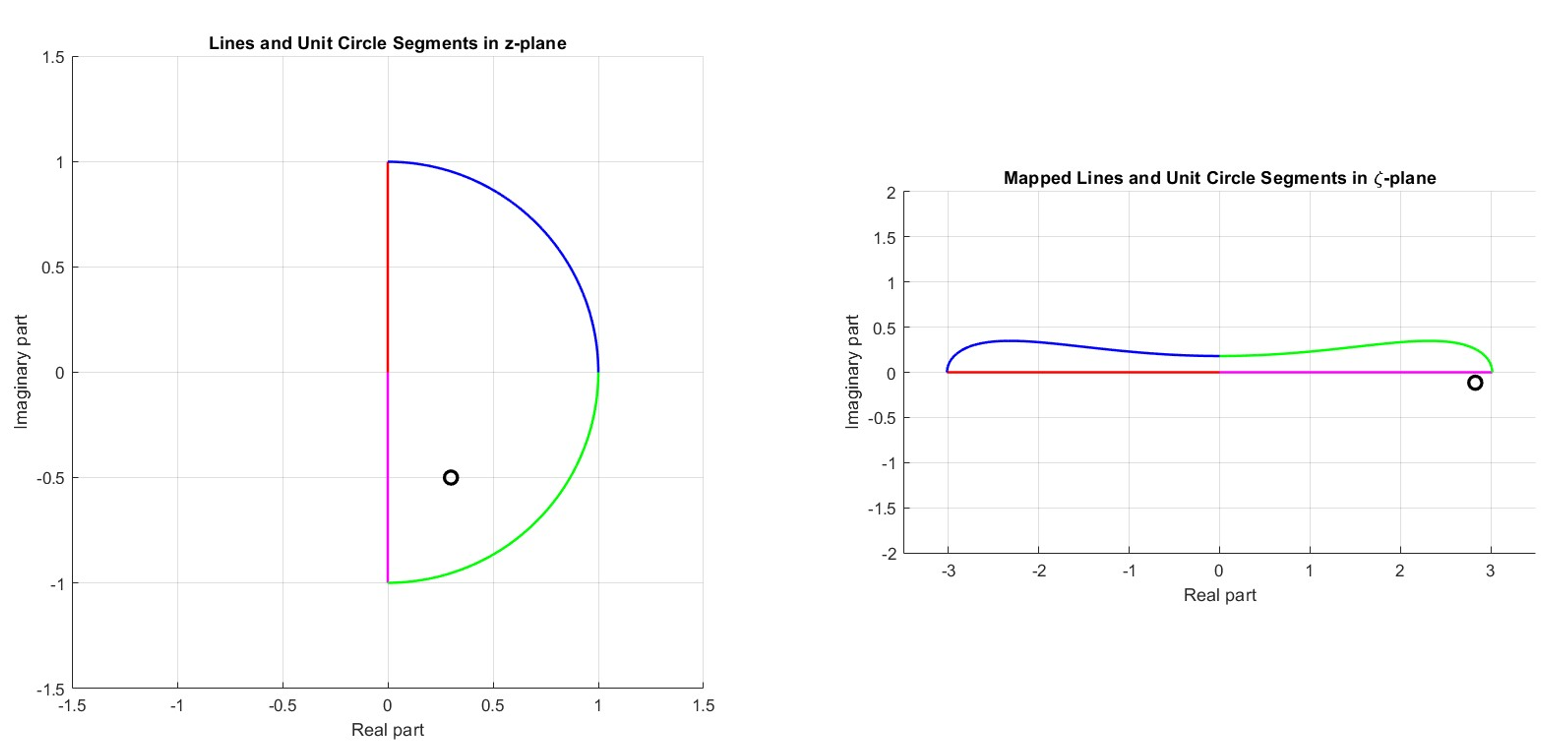
\includegraphics[width=0.75\textwidth]{Figs/crowdy2015_edit.png}
\caption{crowdy15 edit}
\label{fig:example}
\end{figure}

\subsubsection{Mapping Points Inside the Unit Circle to the Lower Half-Circle}

% Given two transformations:

% 1. Mapping points inside the unit circle to the first quadrant:
%    \[
%    \zeta_1 = \sqrt{\left( \frac{1 - \zeta}{1 + \zeta} \right) \cdot i}
%    \]

% 2. Mapping points from the first quadrant to the interior of the lower half-circle:
%    \[
%    \eta_1 = \frac{1 - \eta}{1 + \eta}
%    \]

% To find the relationship between \(\zeta\) and \(\eta\), set \(\zeta_1 = \eta_1\):
% \[
% \sqrt{\left( \frac{1 - \zeta}{1 + \zeta} \right) \cdot i} = \frac{1 - \eta}{1 + \eta}
% \]

% Multiply both sides by \((1 + \eta)\):
% \[
% \sqrt{\left( \frac{1 - \zeta}{1 + \zeta} \right) \cdot i} \cdot (1 + \eta) = 1 - \eta
% \]

% Rearrange to isolate \(\eta\):
% \[
% \sqrt{\left( \frac{1 - \zeta}{1 + \zeta} \right) \cdot i} + \sqrt{\left( \frac{1 - \zeta}{\zeta + 1} \right) \cdot i} \cdot \eta = 1 - \eta
% \]

% Combine \(\eta\) terms:
% \[
% \eta \left( \sqrt{\left( \frac{1 - \zeta}{1 + \zeta} \right) \cdot i} + 1 \right) = 1 - \sqrt{\left( \frac{1 - \zeta}{\zeta + 1} \right) \cdot i}
% \]

Solve for \(\eta\):
\[
\eta = \frac{1 - \sqrt{\left( \frac{1 - \zeta}{\zeta + 1} \right) \cdot i}}{1 + \sqrt{\left( \frac{1 - \zeta}{\zeta + 1} \right) \cdot i}}
\]

\subsubsection{Rewriting as a Hyperbolic Function}

Convert the given mapping formula into a hyperbolic function.

% Given Mapping Formula
% \[
% \eta(\zeta) = \frac{1 - \sqrt{\frac{w}{2}} - i \sqrt{\frac{w}{2}}}{1 + \sqrt{\frac{w}{2}} + i \sqrt{\frac{w}{2}}}
% \]

% where:
% \[
% w = \frac{1 - \zeta}{\zeta + 1}
% \]

% Hyperbolic Function Properties
% The definition of the hyperbolic tangent function is:
% \[
% \tanh(z) = \frac{\sinh(z)}{\cosh(z)} = \frac{e^z - e^{-z}}{e^z + e^{-z}}
% \]

% Transforming the Formula
% Considering the complex logarithm:
% \[
% \log(w) = \log \left( \frac{1 - \zeta}{\zeta + 1} \right)
% \]

% Let:
% \[
% u = \sqrt{\frac{w}{2}}
% \]

% Then the mapping formula can be rewritten as:
% \[
% \eta(\zeta) = \frac{1 - u - iu}{1 + u + iu}
% \]

% Using the Hyperbolic Tangent Function Properties
% We know:
% \[
% \tanh \left( \frac{1}{2} \log \left( \frac{1 - \zeta}{\zeta + 1} \right) \right) = \frac{\sinh \left( \frac{1}{2} \log \left( \frac{1 - \zeta}{\zeta + 1} \right) \right)}{\cosh \left( \frac{1}{2} \log \left( \frac{1 - \zeta}{\zeta + 1} \right) \right)}
% \]
This can be written as:
\[
\eta(\zeta) = \tanh \left( \frac{1}{2} \log \left( \frac{1 - \zeta}{\zeta + 1} \right) \cdot i \right)
\]

% Therefore, by using the properties of the hyperbolic tangent function, we can re-express the original mapping formula in terms of hyperbolic functions.

\subsubsection{further work, $\zeta(\eta)$}
% Square both sides to eliminate the square root:

% \[
% \frac{1 - \zeta}{\zeta + 1} \cdot i = \left( \frac{1 - \eta}{1 + \eta} \right)^2
% \]
% Expanding and rearranging terms:

% \[
% \zeta (1 + \eta)^2 - (1 + \eta)^2 = -i \zeta (1 - \eta)^2 - i (1 - \eta)^2
% \]

% \[
% \zeta (1 + 2\eta + \eta^2) - (1 + 2\eta + \eta^2) = -i \zeta (1 - 2\eta + \eta^2) - i (1 - 2\eta + \eta^2)
% \]

% Combine like terms:

% \[
% \zeta (1 + 2\eta + \eta^2 + i (1 - 2\eta + \eta^2)) = (1 + 2\eta + \eta^2 - i (1 - 2\eta + \eta^2))
% \]

% Factor out \(\zeta\):

% \[
% \zeta (1 + 2\eta + \eta^2 + i (1 - 2\eta + \eta^2)) = (1 + 2\eta + \eta^2 - i (1 - 2\eta + \eta^2))
% \]

% Finally, solving for \(\zeta\):

\[
\zeta = \frac{(1 - i) + (2 + 2i)\eta + (1 + i)\eta^2}{(1 + i) + (2 - 2i)\eta + (1 + i)\eta^2}
\]
\pagebreak
%\renewcommand\bibname{{References}}
%\bibliography{References}
%\bibliographystyle{plain}
\chapter{Potentials of 0$\degree$ Contact Angle Droplets}
\hspace{0em}\indent My supervisor envisions that the local properties of droplets can be revealed within a charge distribution model, which has a geometric scaling similarity to distant droplets. This chapter follows his framework, develops electric potentials for several cases, applies conformal mapping techniques and establishes the non-obvious complex potential of the conducting thin film.

Additionally, it should be noted that the derived functions in this chapter are inconsistent with similar models in \citet{Griffiths_2017} and have been incorporated into more complex scenarios.


\section{Problem Formulation}
\subsection{The Electrode, Dielectric, and Droplet Problem}
\hspace{0em}\indent Consider a droplet situated on a dielectric layer, with electrodes charging the droplet/layer and altering the droplet curve's shape and contact angle, as shown in Figure \ref{fig:sketch electrode}.
    \begin{figure}[H]
        \centering
                \adjustbox{frame=.01pt,frame,margin=.01, color=mycolor}{
        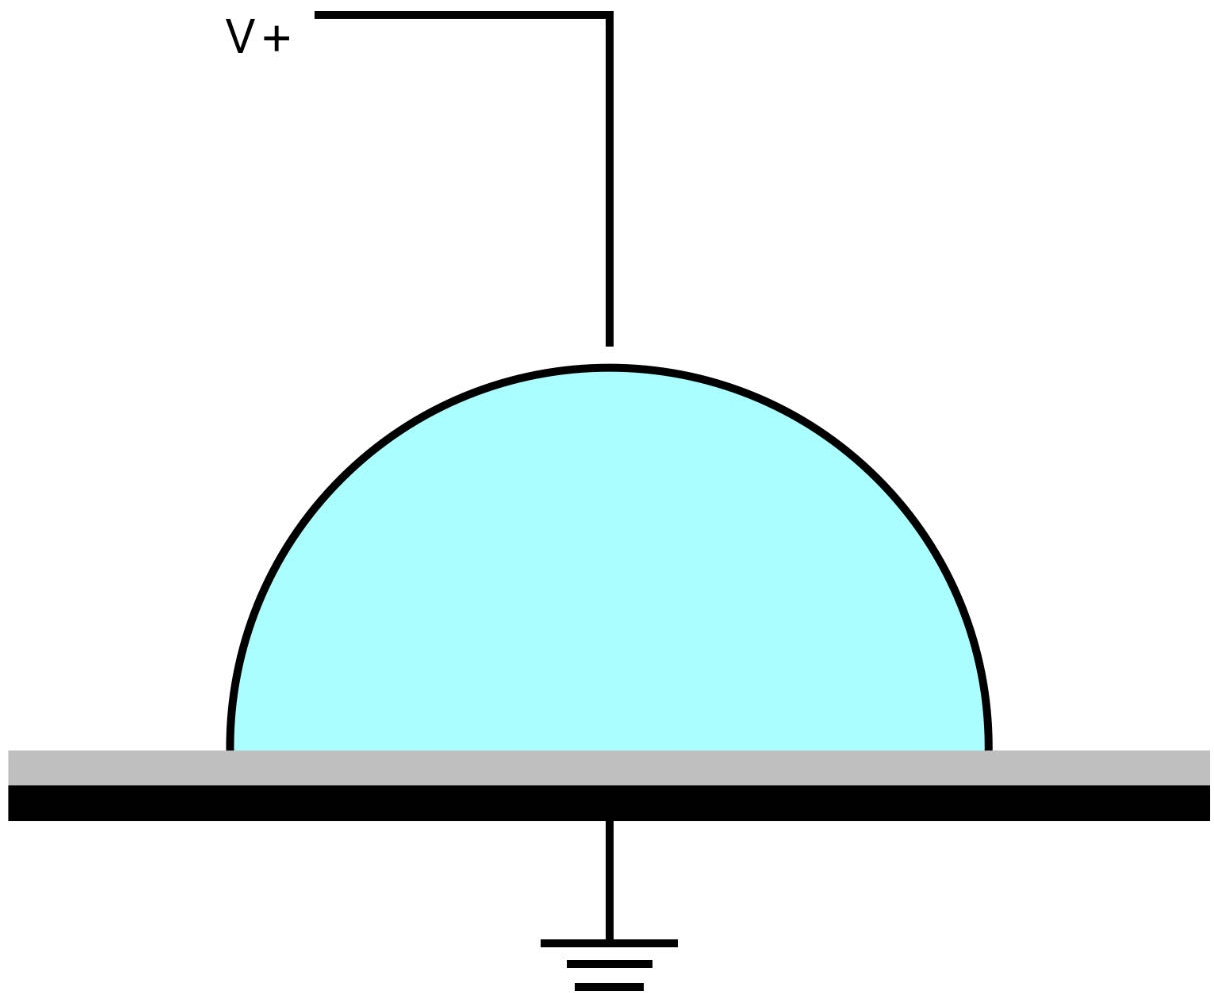
\includegraphics[width=0.7\linewidth]{Figs/sketch eletrode}}
        \caption{\small Sketch of the electrode, dielectric, and droplet problem. The $V_+$ electrode and grounded substrate create a voltage difference across the conducting droplet and layer.}
        \label{fig:sketch electrode}
    \end{figure}
Given the complexity of the functionalisation of the droplet's surface and other related issues, directly obtaining an analytical solution for its electric potential is difficult.

\subsection{The Simplification of the Problem}
\hspace{0em}\indent This study simplifies the problem in several stages. First, when observed from a distance, the droplet's shape degenerates into a thin film with negligible height, which we refer to as a ``slit". The dielectric layer is assumed to be semi-infinite in $-y$ and $\pm x$ directions relative to the slit. Second, the influence of the electrodes is simplified to a point charge, though its precise location and magnitude are not accurately depicted in the following figure, as these parameters may vary. Figure \ref{fig:slit} provides an approximate representation of the simplified Situation.

Additional characteristics of the simplified configuration include the surface charge on the boundary of the dielectric layer, the volume charge within the dielectric, and the voltage at infinity. The latter remains unknown and, at this stage, cannot be constrained in a manner that satisfies the uniqueness theorem (section \ref{thm:uniquenss}).

    \begin{figure}[H]
        \centering
        \adjustbox{frame=0.25pt,frame,margin=0.15,color=mycolor}{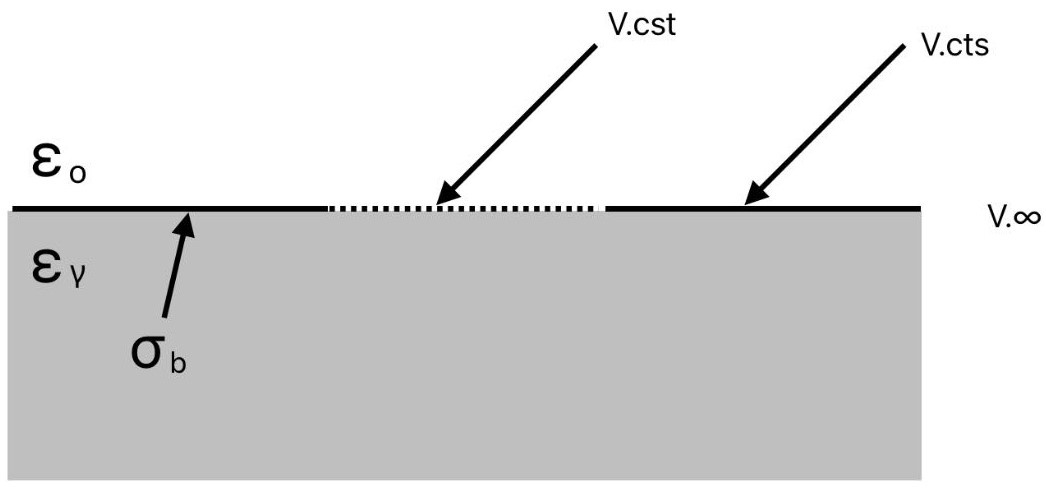
\includegraphics[width=.8\linewidth]{Figs/slit_e.jpg}}
        \caption{\small Thin droplet slit on the dielectric layer. The dashed line represents the slit, while the thick black lines indicate the boundaries of the dielectric and the air above. The shaded areas denote the dielectric, and the upper space of air is left blank. Additionally, $\epsilon_0$ and $\epsilon_{\gamma}$ are the electric permittivity of air and the dielectric, respectively. $\sigma_b$ is the surface charge density of the dielectric layer, with the surface charge density in the air is set to be zero. V.cst indicates the slit is itself an equipotential surface, V.cts means the voltage is continuous along the dielectric-air interface, and V.$\infty$ represents the far-field voltage, which is unknown.\\
        Lastly, it should be noted that we use a point charge to represent the electrodes, which is not shown in the sketch. This point charge is embedded somewhere in the dielectric and varies in magnitude due to the properties of the electrodes.}
        \label{fig:slit}
    \end{figure}
For other properties and coefficients not explicitly included in the sketch, we can now establish the boundary conditions:
\begin{itemize}
    \item All charges of the conductive droplet $\Omega$ are distributed along the boundary of the droplet.
    \vspace{-0.5em}
   \[\int_{\partial \mathcal{D}} \sigma_{\partial\Omega} \df l = Q_{\Omega}\vspace{-0.5em}
   \]
    \item There is an induced volume charge density $\rho$ at $\vec{r_0}$ in the dielectric, where the embedded point charge is located.
    \[
    \epsilon_0\nabla\cdot \mathbf{E}=\frac{q}{\epsilon_r}\delta(\vec{r}-\vec{r}_0)%\vspace{-1em}
    \]
    \item Except for the location of the embedded point charge, all induced charges in the dielectric $\mathcal{D}$ are distributed along the boundary of the dielectric and the air.
    \vspace{-.5em}
     \[\nabla\cdot \mathbf{E}=0\hspace{1em}\text{s.t. in }\mathcal{D}\setminus \{\partial \mathcal{D} \cup \vec{r}_0\}\vspace{-1em}\]
    \item The voltage of the conducting droplet is constant.
    \vspace{-0.5em}
    \[V(\Omega)=Constant\vspace{-1em}\]
    \item The voltage is continuous on the boundary $\partial \Omega$. The voltage $V^{(b)}$ represents that in the dielectric, and the air above has a voltage $V^{(a)}$ .
    \begin{equation}\label{eqn:v.cts}
\left.V^{(a)}\right|_{\partial\mathcal{D}^+}=\left.V^{(b)}\right|_{\partial\mathcal{D}^-}        
    \end{equation}
\end{itemize}
\vspace{-.5em}
\hspace{0em}\indent Yet some uncertain properties at this stage include:
\begin{itemize}
    \item There may be induced charges at the boundary $\partial\mathcal{D}$, caused by the presence of free charge(the point charge). let $\l^o$ be a small closed loop across the boundary $\partial\mathcal{D}$; Gauss's Law states that 
    \[\oint_{l^o} -\epsilon \nabla V\cdot\hat{n}\df l = \pi r^2\sigma_b\]
    or in terms of $\vec{E}$, since the boundary lies along the $x$-axis, only the $y$ component of $\vec{E}$ contributes:
    \begin{equation}\label{eqn:gauss}
    \epsilon_0 E^{(a)}_y-\epsilon_\gamma E^{(b)}_y=\sigma_b   
    \end{equation}
    
    However, charge distributions with no induced charge on the boundary between the dielectric and the space above do exist, as a later case shows.
    
    \item We are generally uncertain about the exact behaviour at infinity.  Besides the far-field voltage of a point charge, the voltage at infinity does not necessarily decrease, the semi-infinite dielectric may contribute.

    \item The equipotentials around the slit are unknown, as are those around the two cusps. Additionally, the induced charge of the slit mixes with that of the dielectric at the slit's lower boundary line\(\partial\Omega \cap \partial\mathcal{D}\).
\end{itemize}

although the droplet's height is ignored, the electric potential of the simplified problem remains challenging due to the boundary conditions.

\subsection{Apply the Joukowski Transformation}\label{cpt:jkw}

\hspace{0em}\indent The Joukowski transformation maps the slit to a disc. If we can determine an appropriate electric potential for the embedded disc, dielectric, and point charge scenario, we can use the inverse map to address the cusps. However, this approach introduces a new challenge due to the asymmetric dielectric geometry relative to the y-axis, as outlined in Figure \ref{fig: maped disc}.

\begin{figure}[H]
    \centering
    \adjustbox{frame=0.25pt,frame,margin=0.15,color=mycolor}{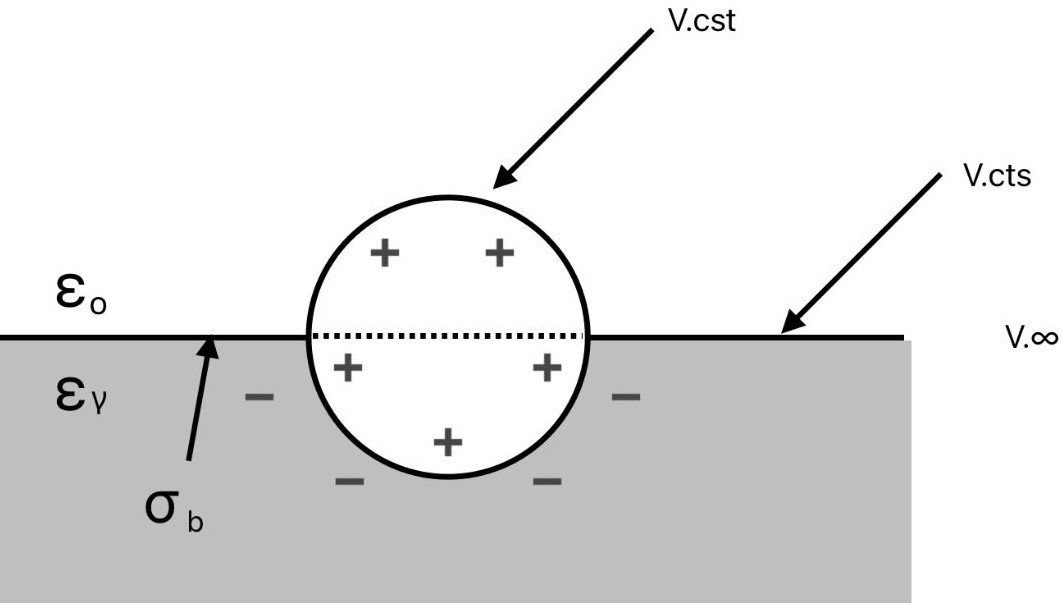
\includegraphics[width=.8\linewidth]{Figs/disk.jpg}}
    \caption{\small The problem corresponds to the Joukowski transformation. In addition to the previously included parameters, the $+$ and $-$ signs represent the surface charge distributions on the disc and the dielectric boundary in contact with it.}
    \label{fig: maped disc}
\end{figure}
the corresponding boundary conditions include:
\begin{itemize}

    \item $\nabla^2 w = 0$ except at boundary lines and the location of the point charge, where $w$ is the complex potential.
    
    \item At $|\zeta|\leq1$, $\Im [w]=0$. This represents the $V(\Omega)$ condition.
    
    \item at $\zeta\in\mathbb{R}$, $\Im [w_a]=\Im [w_b]$, representing the continuous voltage condition on the boundary in the complex plane.
    
\end{itemize}
Hence, we are eventually facing a Laplace equation/Poisson equation problem.

\section{Analyzing the Component Electrical Models}
\subsection{Charged Disc Embedded in Dielectric: A Point Charge-like Electric Field}\label{cpt:charged disc}
\hspace{0em}\indent Consider a disc of radius $R=1$, charged with $q$, embedded in a semi-infinite dielectric. let $\theta_s$ be the arc of the disc in contact with the dielectric.

The dielectric structure is symmetric about $\theta_s$, which corresponds to the right angle at the contact point in Figure \ref{fig:disk in D}. However, it allows for variation in how much the disc is embedded, as measured by the parameter $\theta_s$.
\begin{figure}[H]
    \centering
    \adjustbox{frame=0.25pt,frame,margin=0.15pt,color=mycolor}{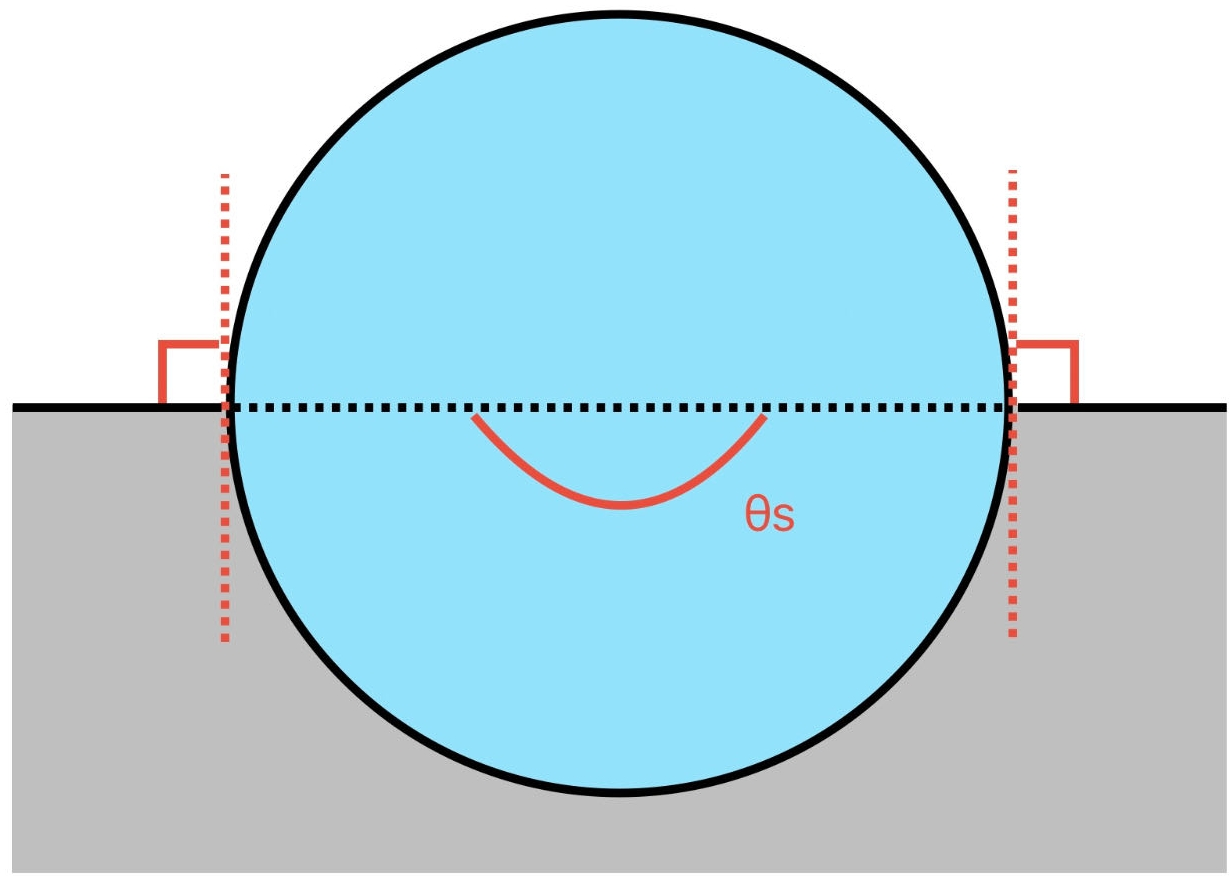
\includegraphics[width=0.46\linewidth]{Figs/sketch disk embedded right.jpg}}\hfill
    \adjustbox{frame=0.25pt,frame,margin=0.15pt,color=mycolor}{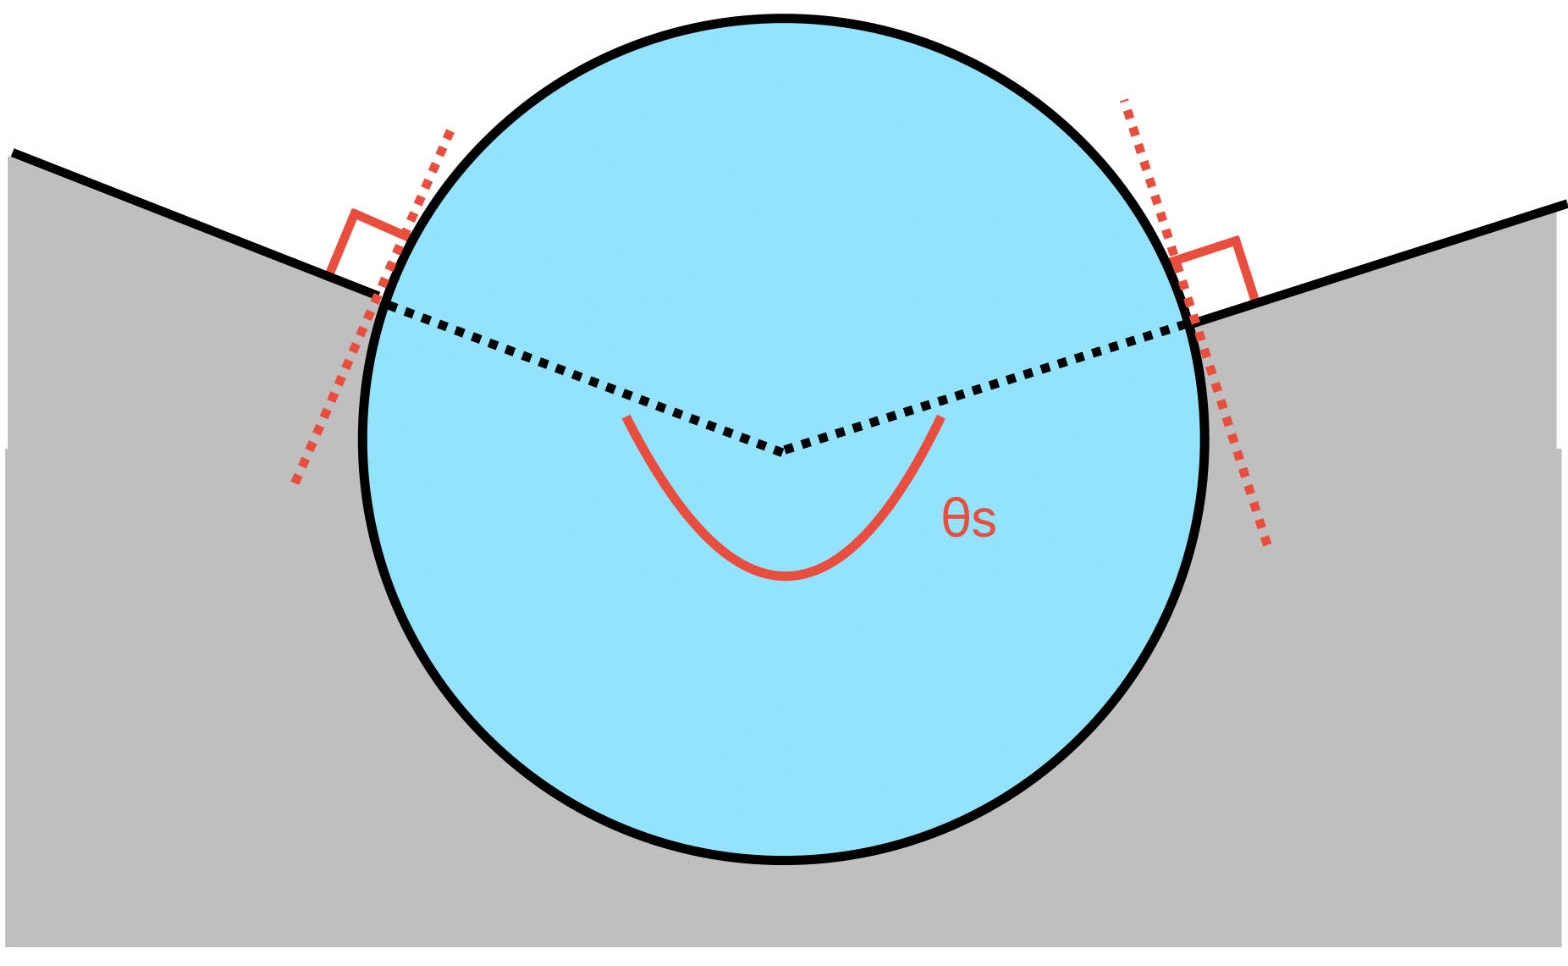
\includegraphics[width=0.531\linewidth]{Figs/sketch disk embedded angle.jpg}} % Side by side images
    
    \caption{\small Two cases are presented where the disc is embedded in a dielectric, measured by $\theta_s$. The left figure shows the case where $\theta_s=\pi$, while the right figure depicts a different $\theta_s$. It is found that the electric fields of the cases differ based on $\theta_s$.}
    \label{fig:disk in D}
\end{figure}

Postulate that the far-field voltage is 
\[V_{\infty}=  \frac{q'}{2\pi\epsilon_0} \log r\]
where $q'\not\equiv q$ is some magnitude of charge. If the voltage satisfies the necessary local boundary conditions, we can be confident that this is the correct voltage for the configuration according to the uniqueness theorem (\ref{uniqueness}).

On the boundary between the droplet and the dielectric, $R=1, \theta\in(0\footnote{Let the point where the dielectric contacts the disc from the left be the zero angle.}, \theta_s)$. According to equation (\ref{eqn:die surf q}),
\[
\sigma_b = \vec{P}\cdot\hat{n}=\epsilon_0 \chi_e E_{\hat{r}}
\]
where\footnote{Note that along the arc, the normal direction of the dielectric boundary points toward the origin. Let the disc be positively charged; the electric field of the disc points outward. Also, note that the sum of the induced surface charge (from both the dielectric and the disc) is positive, with its own electric field lines pointing outward, which is why there are two minus signs in equation (\ref{eqn:surf dq}). }
\begin{equation}\label{eqn:surf dq}
    E_{\hat{r}} = -E_{q} - \frac{\sigma_b}{2 \epsilon_0}  
\end{equation}
Hence
\[
\sigma_b= \epsilon_0 \chi_e \left( -\frac{q}{2 \pi R \epsilon_0} - \frac{\sigma_b}{2 \epsilon_0} \right)
\Longrightarrow \sigma_b = -\frac{q}{2 \pi R} \cdot \frac{2 \chi_e}{2 + \chi_e}
\]
Postulate that the surface charge density in the dielectric\footnote{At the contact line of the dielectric and the disc, the total surface charge density is the sum of both.} on the arc at $R=1$ is uniformly $\sigma_b$, then the total surface charge $q_s$ is
\[\sigma_b \int^{\theta_s} R\df\theta= -q \frac{2 \chi_e}{2 + \chi_e}\cdot\frac{\theta_s}{2 \pi} =q_s\]
let $\theta_s=\pi$ in our case, the total charge $q_t$ of the system is then
\begin{equation}\label{eqn:disk,d,qt}
    q_t=q+q_s=q(1-\frac{1}{2}\frac{2\chi_e}{2+\chi_e})=q\frac{2}{2+\chi_e}\leq q
\end{equation}
The electric field is unique everywhere, regardless of whether it is in the dielectric or not:
\[
\vec{E}=\frac{q_t}{2\pi\epsilon_0 r}\hat{r}=\frac{q}{2\pi\epsilon_0 r}\frac{2}{2+\chi_e}\hat{r}
\]
and the voltage is:
\[
v=\frac{1}{2\pi\epsilon_0}\frac{2q}{2+\chi_e}\log r
\]
The electric field is symmetric about the origin; its field lines parallel to the dielectric boundary along $\pm x$. Hence, the dielectric contains no surface charge other than $\sigma_b$ on the arc.

The surface charge distribution on the disc, $\sigma_d$, is then
\begin{align*}
\sigma_d&= \begin{cases}q_t/\pi &, \theta\in(0,\pi) \\
|\sigma_b| + q_t/\pi &,  \theta\in(\pi,2\pi)\end{cases}
\end{align*}

\subsection{Point Charge Embedded in Dielectric: Different Electric Fields in Various Regions}\label{cpt:charge in die}
\hspace{0em}\indent For a point charge embedded in a dielectric below the $x$-axis, the three types of charges in this setup are the free charge, the induced volume charge, and the induced surface charge.

The free charge $q_f$ is simply the point charge $q$. The point charge induces a volume charge density $\rho_b$ at $\vec{r}_0(x,y) = (0, -d)$, \[q_b=\int_\mathcal{V}\rho_b\Longleftrightarrow \rho_b = q_b\delta(\vec{r}-\vec{r}_0)
\]
and an induced surface charge density $\sigma_b$.

The two quantities need to be determined to satisfy the following boundary conditions, equation (\ref{eqn:v.cts}), which ensures continuity in voltage, and equation (\ref{eqn:gauss}), which applies Gauss's Law to the surface charge density.

The electric field consists of two different components. For the voltage inside the dielectric, we treat the charge and the induced volume charge field as a single entity $q$, Gauss's Law provides:
\[
V = \frac{q}{2\pi\epsilon} \log(r - r_0)
\]
where $\epsilon$ is the permittivity.

By method of Image, we replace the dielectric with induced charges and treat all charges as if they were in a vacuum, using $\epsilon_0$, hence 
\[V_{q}=\frac{q}{2\pi\epsilon_0} \log(r-r_0)\]
and
\[V_{q_b}=\frac{q_b}{2\pi\epsilon_0} \log(r-r_0)\]
By equation (\ref{eqn:P}), $\vec{P}=\epsilon\chi_e \vec{E}$, and equation (\ref{eqn:rho_b}), $\rho_b\coloneqq-\nabla\cdot\vec{P}$,
\[q_b\coloneqq\int_{\mathcal{V}} \rho_b\delta (\vec{r}-\vec{r}_0)=-\frac{\chi_e}{1+\chi_e}q\Longrightarrow q+q_b=\frac{1}{1+\chi_e}q=\frac{q}{\epsilon_r}
\]
the two voltages sum to
\[
V=V_q+V_{q_b}=\frac{1}{2\pi\epsilon_0}\frac{q}{\epsilon_r}\log (r-r_0)=\frac{1}{2\pi\epsilon_0}\frac{q}{\epsilon_r}\log\sqrt{(x-0)^2+(y--d)^2}
\]
the electric field pointing $\hat{y}$ is
\[
E_y=-\frac{\partial V}{\partial y}=\frac{1}{2\pi\epsilon}\frac{q}{\sqrt{(x)^2+(y+d)^2}}\frac{1}{\sqrt{(x)^2+(y+d)^2}}\frac{1}{2}2(y+d)=\frac{1}{2\pi\epsilon}\frac{q(y+d)}{x^2+(y+d)^2}
\]
at $y=0$
\[
E_q=\frac{1}{2\pi\epsilon}\frac{qd}{x^2+d^2}=\frac{1}{2\pi\epsilon_0}\frac{1}{1+\chi_e}\frac{qd}{x^2+d^2}
\]
by equation (\ref{eqn:ed.line}), surface charge density satisfies
\[
E_\sigma=-\frac{\sigma_b}{2\epsilon_0}
\]
and by equation (\ref{eqn:rho_b}), $\sigma_b=\vec{P}\cdot\hat{n}=\epsilon_0\chi_e\vec{E}\cdot\hat{n}$, from the two we find
    \[    \sigma_b=\epsilon_0\chi_e\left(E_q+E_{\sigma}\right)=\epsilon_0\chi_e\left(\frac{1}{2\pi\epsilon_0}\frac{1}{1+\chi_e}\frac{qd}{x^2+d^2}-\frac{\sigma_b}{2\epsilon_0}\right)\Longrightarrow
        \frac{2+\chi_e}{2}\sigma_b=\frac{1}{2\pi}\frac{\chi_e}{1+\chi_e}\frac{qd}{x^2+d^2}
    \]
hence the induced surface charge density of the dielectric, on $y=0$, is
\[
\sigma_b=q\frac{\chi_e}{1+\chi_e}\frac{1}{2+\chi_e}\frac{ d / \pi}{x^2+d^2}
\]
\subsection{Dielectric Shielding and the Difference from \citeauthor{Griffiths_2017}}\label{cpt:shield}
\hspace{0em}\indent After deriving the electric properties for the models above, we find that our results are inconsistent with similar cases in Chapter 4 of \citet{Griffiths_2017}. In Example 4.5 on page 187, the textbook derives the case of a metal sphere charged $Q$, surrounded by dielectric of finite radius and finds that in the region $\vec{r}>\vec{r}_{\mathcal{D}}$,
\[E_{textbook}\sim Q/\epsilon_0\] 
However, using our derivation method, the electric field is found to be
\[E= \frac{1}{4 \pi r^2}\frac{Q}{\epsilon_0}\frac{2}{2+\chi_e}\] 
which is smaller by a factor $\frac{2}{2+\chi_e}$ compared to the textbook result. The other two similar cases from \citet{Griffiths_2017} are Problem 4.35, concerning a point charge in a spherical dielectric; and Problem 4.38, regarding a conducting sphere embedded in a dielectric\footnote{See \citet{Griffiths_2017}, Ex. 4.5, p. 187 and Problem 4.35, p. 206, for reference.}.

In these cases, the textbook derives without considering certain surface charge densities. All our results are smaller by a factor of $\frac{2}{2+\chi_e}$, and the details of calculations are omitted here.

Hence we need to examine carefully if they match the required local boundary conditions in our situation. For the point charge in the dielectric case, we check whether the integral of the surface charge density, $q_s$, cancels out the induced volume charge $q_b$
\[
q_s\coloneqq\int_S \sigma_b \df a \Longrightarrow \int_\mathbb{R}\sigma_b \df x=q\frac{1}{1+\chi_e}\frac{\chi_e}{2+\chi_e}\frac{d}{\pi}\int_\mathbb{R}\frac{1}{x^2+d^2}\df x=...\frac{d}{\pi} \frac{\pi}{d}=q\frac{\chi_e}{1+\chi_e}\frac{1}{2+\chi_e}
\]
Yet the amount of induced volume charge is:
\begin{equation}\label{eqn:sigma_b}
q_b=\int_\mathcal{V}-\nabla\cdot\vec{P}=-\nabla\cdot\epsilon_0\frac{\chi_e}{\epsilon}\vec{D}=- q\frac{\chi_e}{1+\chi_e}    
\end{equation}
we observe that $q_s \neq q_b$. If they were equal, it would almost imply that, when observed from the outside, the dielectric appears to have no effect\footnote{Which is the scenario presented in \citet{Griffiths_2017} examples, and is not in this thesis. The derivation follows.}. Since this is not the case, we must locate the surplus charge to determine the dielectric's actual effect in the situation. 

The voltage below is the potential due to three point charges. The charges $q_f$ and $q_b$ at $(x,y) = (0,-d)$, sum to
\[
q_r=q_f + q_b = (1-\frac{\chi_e}{1+\chi_e} )q =\frac{1}{1+\chi_e}q=\frac{q}{\epsilon_r}
\]
and the induced surface charge sums to $q_s$. We locate it at $(x,y)=(0,d)$. The voltage below the $x$-axis is therefore
\begin{align*}
    V_{below}&=\frac{1}{2\pi\epsilon_0}\left(q_r\log\sqrt{x^2+(y+d)^2} +q_s\log\sqrt{x^2+(y-d)^2}\right)
    \\&=\frac{q}{2\pi\epsilon_0}\left(\frac{1}{\epsilon_r}\log\sqrt{x^2+(y+d)^2} +\frac{\epsilon_r-1}{\epsilon_r}\frac{1}{\epsilon_r+1}\log\sqrt{x^2+(y-d)^2}\right)
    \\&=\frac{q}{2\pi\epsilon_0}\left(\frac{1}{\chi_e +1}\log\sqrt{x^2+(y+d)^2} +\frac{\chi_e}{1+\chi_e}\frac{1}{2+\chi_e}\log\sqrt{x^2+(y-d)^2}\right)    
    \\&=\frac{q}{2\pi\epsilon_0\epsilon_r}\left(\log\sqrt{x^2+(y+d)^2} +\frac{\chi_e}{2+\chi_e}\log\sqrt{x^2+(y-d)^2}\right)    
    \end{align*}

For the voltage above the $x$-axis, locate $q_s$ at $(x,y) = (0,-d)$, while the other two remain at their original positions. The three charges sum to
\[q_t=
q_o+q_b+q_s=\frac{q}{\epsilon_r}+\frac{q}{\epsilon_r}\frac{\chi_e}{2+\chi_e}=\frac{q}{1+\chi_e}\frac{2+2\chi_e}{2+\chi_e}=\frac{2q}{\chi_e+2}
\]
hence the voltage is
\[
V_{above}=\frac{1}{2\pi\epsilon_0}\frac{2 q}{({\chi_e+2})}\log\sqrt{x^2+(y+d)^2}=\frac{q}{\pi\epsilon_0}\frac{1}{(\epsilon_r+1)}\log\sqrt{x^2+(y+d)^2}
\]
Moreover, check if Gauss's Law satisfies
\begin{align*}
\frac{\partial V_{above}}{\partial y}-\frac{\partial V_{below}}{\partial y}&=\frac{q}{2\pi} \left( \frac{2}{\epsilon_r + 1} \frac{y + d}{x^2 + (y + d)^2} - \frac{1}{\epsilon_r} \frac{y + d}{x^2 + (y + d)^2} -\frac{1}{\epsilon_r} \frac{\epsilon_r-1}{\epsilon_r+1}\frac{y - d}{x^2 + (y - d)^2}\right)   
\end{align*}
at $y=0$
\begin{align*}
\left.\frac{\partial V_{upper}}{\partial y}-\frac{\partial V_{lower}}{\partial y}\right|_{y=0}&=\frac{q}{2\pi} \frac{d}{x^2 + d^2}\left( \frac{2}{\epsilon_r + 1} - \frac{1}{\epsilon_r} +\frac{1}{\epsilon_r}\frac{\epsilon_r-1}{\epsilon_r + 1}  \right) \\
    &=\frac{q}{2\pi}  \frac{d}{x^2 + d^2}  \frac{2\epsilon_r -\epsilon_r -1+\epsilon_r -1}{\epsilon_r(\epsilon_r + 1)} \\
    &=\frac{q}{2\pi}  \frac{d}{x^2 + d^2} \frac{2\epsilon_r -2}{\epsilon_r(\epsilon_r + 1)} \\
    &=\frac{q}{\pi}  \frac{d}{x^2 + d^2} \frac{\epsilon_r -1}{\epsilon_r(\epsilon_r + 1)}=\frac{q}{\pi}  \frac{d}{x^2 + d^2}\frac{\chi_e}{\chi_e +1}\frac{1}{\chi_e +2}
\end{align*}

It matches $\sigma_b$ in equation \ref{eqn:sigma_b}; Gauss's Law is fulfilled\footnote{For further confirmation, see a related problem at \citet{Griffiths_2017} Ex 4.25, p. 207.}. 

The voltage $V_{above}$ describes how the dielectric affects the surroundings. We observe that the apparent magnitude of the charge $q_s$ varies, yet it retains the form of a point charge with a fixed location. Consequently, the problem of the point charge, dielectric, and droplet reduces to that of a point charge field, differing only in the charge magnitude, which is advantageous.

Furthermore, an interesting phenomenon was observed: the voltage outside the dielectric is not as commonly expected, as though the dielectric had no effect at all:
\[
V_{expected}=\frac{q}{2\pi\epsilon_0}\log\sqrt{x^2+(y+d)^2}
\]
implies the dielectric leaves no effect on the external  region\footnote{If this were true, we receive two electric signals from the same charge, once sent from the vacuum, and once enclosed by dielectric before sending. There will be no difference between the two.}.  

Our derivation shows the quantity of a charge embedded in a dielectric, as seen from outside, is less than it actually is.
\[
\frac{V_{upper}}{V_{expected}}=\frac{q}{\pi\epsilon_0(\epsilon_r+1)} / \frac{q}{2\pi\epsilon_0}=\frac{2}{1+\chi_e+1}\leq 1\vspace{3em}
\]
Physically, this claims the dielectric shields some of the electric energy of embedded charges, which sounds plausible. The equipotentials of the point charge embedded in the dielectric are as follows.
\begin{figure}[H]
    \centering
    \adjustbox{frame=0.25pt,frame,margin=0.15,color=mycolor}{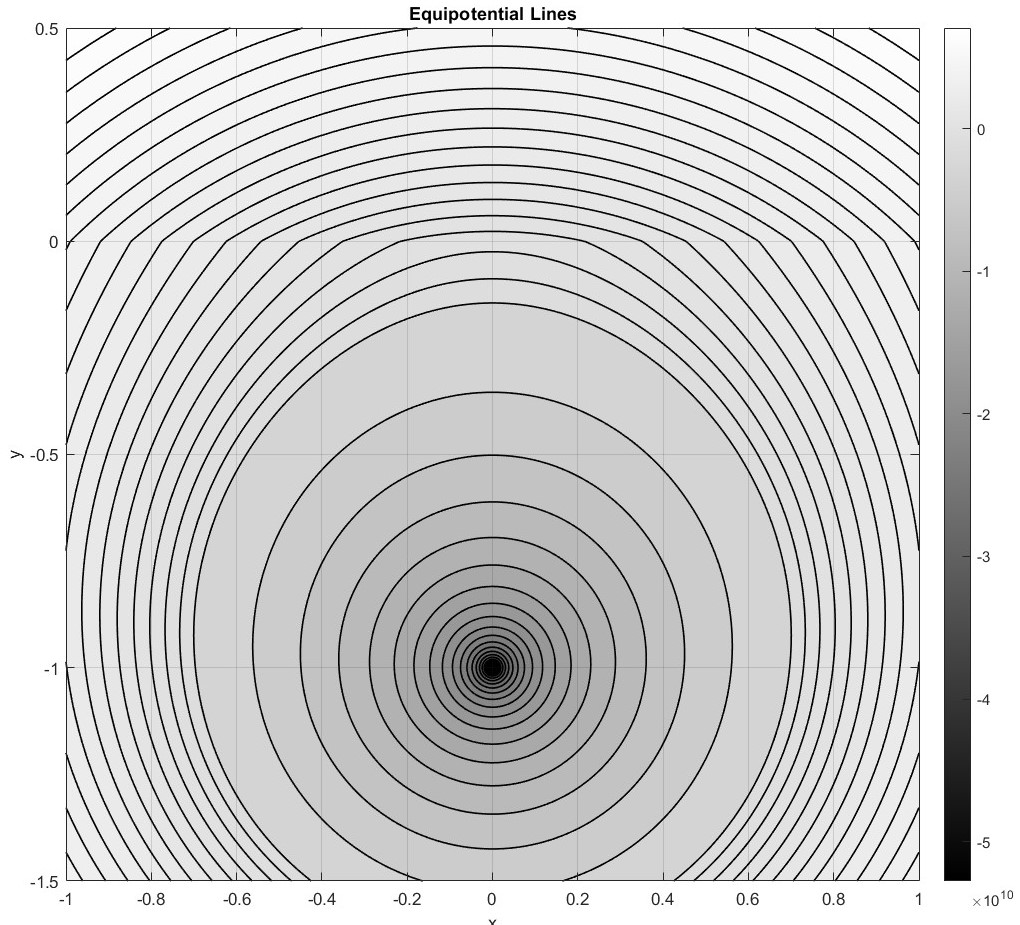
\includegraphics[width=1.\linewidth]{Figs/dieletic potential.jpg}}
    \caption{\small The equipotentials of a point charge embedded in the dielectric exhibit a noticeable change in direction at \(y=0\), which is the boundary between the dielectric and the air above. This indicates that the electric field is disrupted while the potential remains continuous due to the induced surface charge. In the region \(y>0\), the potential forms concentric circular equipotential lines created by a charge located at \(y=-d\), which has a smaller magnitude than the actual charge.
 }
    \label{fig:enter-label}
\end{figure}

In the case of a charged disc embedded in a dielectric, we find that $q_t\leq q$ in equation (\ref{eqn:disk,d,qt}), which also demonstrates the shielding effect.
\section{The Potential of the Charge, Dielectric, and Disc Problem}
\subsection{The Complex Potential of the Disc}
\hspace{0em}\indent For a typical complex potential, it is free to use either the real or imaginary part to be the voltage. However, we will set the imaginary part as the voltage, because we require $r=1$ to be an equipotential, $\Im \left[w(|\zeta|=1)\right]=0$ , by adding $\overline{w}(\zeta^{-1})$. The complex potential of the charge is\vspace{-1.em}
\[
w_0(\zeta)=\im \log (\zeta-\zeta_0)\vspace{-1.5em}
\]
and adding
\[
\overline{w_0}(\frac{1}{\zeta}) = -\im \log (\frac{1}{\zeta}-\Bar{\zeta_0})
\]
This generates two physical entities: a sink $-\im\log (1-\zeta\zeta_0)$ at $1/\overline{\zeta_0}$ , and a source $\im\log(\zeta)$ at $\zeta = 0$ . For a point charge at \(\zeta_\alpha\) and for the unit circle to be an equipotential, two extra charges of opposite sign must be added.

\subsection{The Induced Charges of the Dielectric}
% The effect of the charges in the dielectric is investigated using conformal mapping and yields surprising results that may help understand the properties of this geometric form of a dielectric.
\hspace{0em}\indent 
The disc induces two charges inside, which may affect the dielectric and therefore require investigation. The charge at \(\zeta = 0\) does not influence the dielectric except on the arc, as proved in section (\ref{cpt:charged disc}). However, the charge at \(1/\overline{\zeta_\alpha}\) may induce surface charge in the dielectric. 

Suppose the charge in the disc off the origin induces a charge in the dielectric; it will induce two more charges inside the disc, the twice-induced charges. As this process continues, the voltage will evolve into a series\vspace{-0.5em}
\[
q\log (\zeta-\zeta_{\alpha})+\frac{q}{\epsilon}\log (\zeta-\zeta_1)+\frac{q}{\epsilon^2}\log (\zeta-\zeta_2)+...\vspace{-0.5em}
\]

The dielectric is not flat, and we are uncertain about the possibly induced charge. To determine the possible induced charge, map the surface of the dielectric to a flat one, with
\[\zeta=z-\sqrt{z^2-1}\]
\begin{figure}[H]
    \centering
    \adjustbox{frame=0.25pt,frame,margin=0.15,color=mycolor}{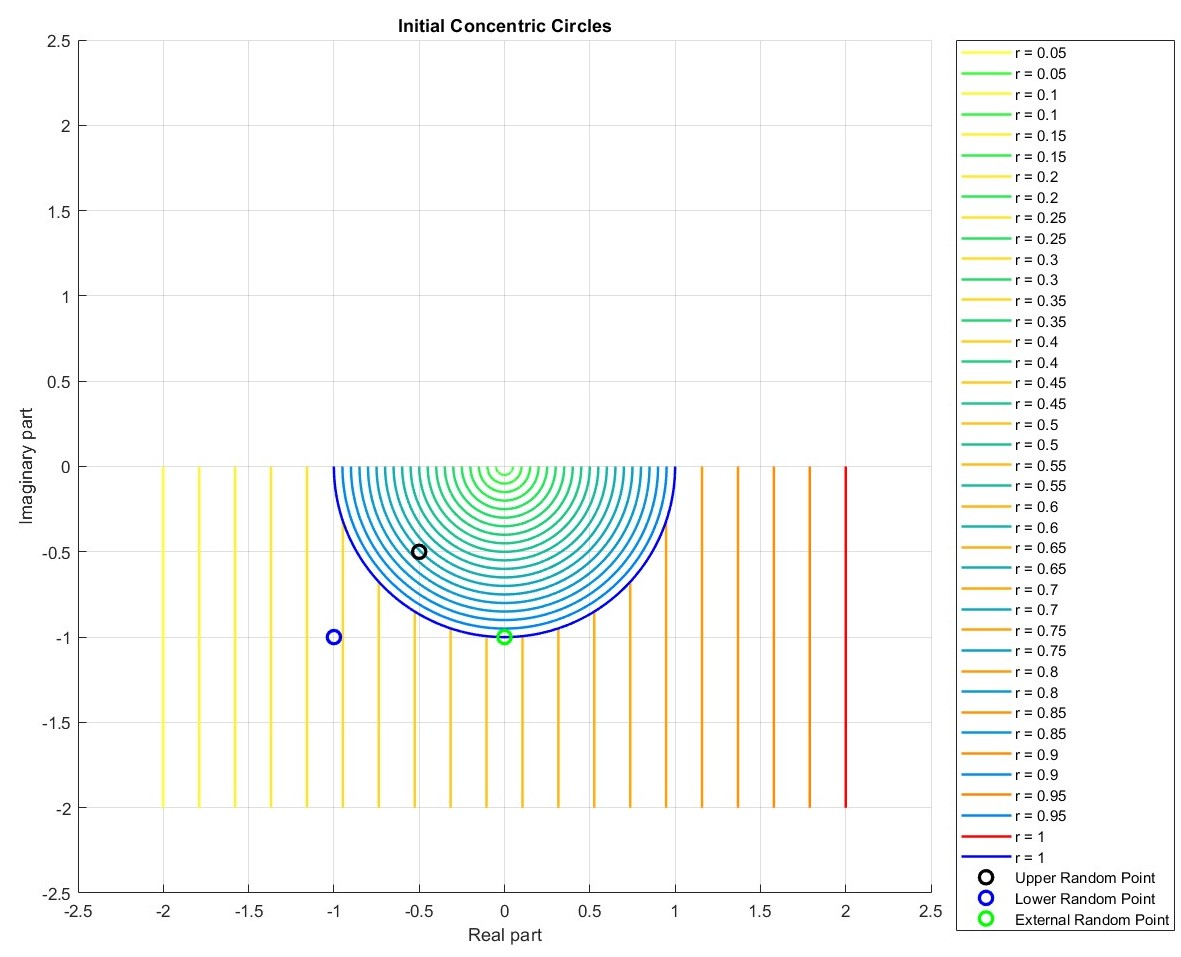
\includegraphics[width=0.493\linewidth]{Figs/semi circle and dieletric}}\hfill
    \adjustbox{frame=0.25pt,frame,margin=0.15,color=mycolor}{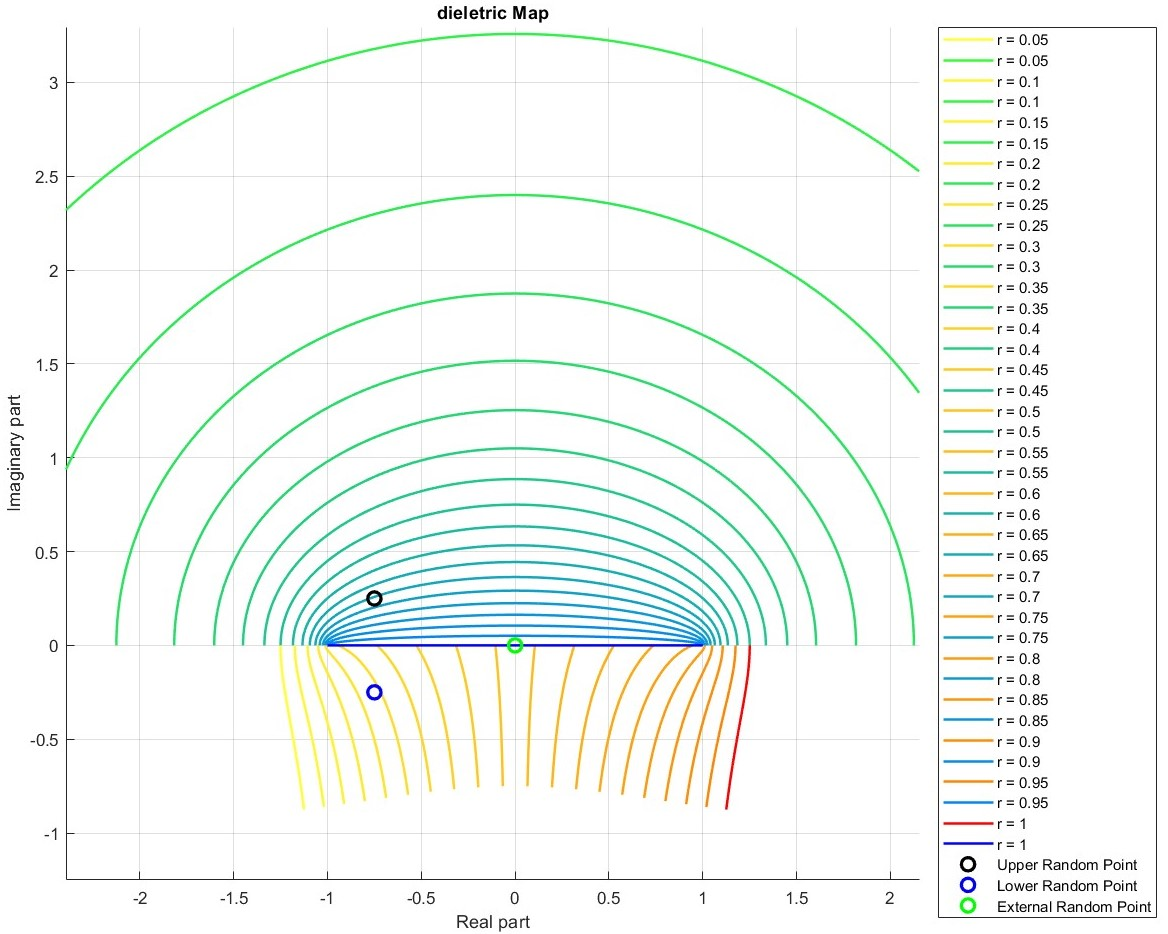
\includegraphics[width=0.5\linewidth]{Figs/map flat dieletric}} % Side by side images
    \caption{\small The point charge (the blue circle) and one of the induced charges (the black circle) in the disc. The left figure is the $\zeta$ plane, the right figure is the $z$ plane. The lower semi-circle (green and blue lines) map to the $y>0$ space, and the dielectric (yellow and red lines) map to $y<0$. The origin $\zeta=0$ maps to $\infty$, which fits the physical condition of the dielectric.\\
    Moreover, The dielectric area is compressed, and physically, $\epsilon$ may change, hence the dielectric is not linear anymore. This possible effect is ignored. 
}
    \label{fig:induce charge map}
\end{figure}

From the right figure of the $z$ plane, we see that the source charge (the blue circle) induced a charge (the black circle). For a point charge at $\zeta_{\alpha}=(-1-\im)$ in the dielectric, the corresponding induced charge inside the disc is at\vspace{-1.em}
\[\zeta_{o}=1/\zeta_{\alpha}=-\frac{1}{2}-\frac{1}{2}\im\vspace{-1.em}\]
and it maps to
\[
z_{o}=\frac{\zeta_{0}}{2}+\frac{1}{2 \zeta_{o}}=-\frac{3}{4}+\frac{1}{4}\im\]
Since the mapped dielectric is flat, take the conjugate to find $z_d=-\frac{3}{4}-\frac{1}{4}\im$, this is the location of the possibly twice-induced charge. The inverse map finds the twice-induced charge's location on the $\zeta$-plane is
\[
\zeta_d=z_d-\sqrt{z^2-1}=-1-\im
\]
This is where the source charge is located; hence, there will be no continuous charge generation.

The two induced charges in the complex equation are located within a conducting disc, where a real free charge cannot reside from a physics perspective. Therefore, they should represent an cumulative effect of the surface charges in the disc and induce no further charges.

\iffalse
This means the conformal mapping captures the physics property of the geometry of the dielectric. A further question is how the equipotential line requirement is fitted, as the dielectric area is rather ordinary. It will be discussed later.

The next question is, will the charge in the unit disc induce a charge in the dielectric? verified via conformal mapping, if it does, the location will be the location of the source charge. 


\begin{itemize}
    \item The induced charge of the source charge will not lie within the disc but will instead be projected onto the opposite side of the disc, and it generates a corresponding charge distribution within the conductive disc.
    \item The potential inside the dielectric is the superposition of the potentials generated by the source charge, its image charge, and the corresponding charge distribution within the disc.
    \item The potential outside the dielectric is equivalent to the potential generated by a smaller charge together with a conductive disc.
    \item The charges within the disc will not generate induced charges (either in the dielectric or elsewhere). There will be no free charges located inside the conductor, and this charge is a substitute for several induced surface charge distributions and therefore will not generate further induced charges.
\end{itemize}
Therefore, the internal voltage of the dielectric we proposed earlier is sufficient, with limited charge adjustment and compensation.

\fi

\subsection{The Potential on the $\zeta$-plane}\label{cpt:pot_zeta}
\hspace{0em}\indent The voltage has two parts, according to section (\ref{cpt:shield}). Assume the voltage in the air is the sum of a point charge (magnitude to be determined) and the induced charges in the disc. The complex potential of above is found to be\vspace{-1em}
\begin{equation}\label{eqn:w_up}
    w_{+}(\zeta) = \frac{q}{\pi \epsilon_0}\frac{1}{\epsilon_r+1} \im \left[ \log(\zeta - \zeta_0) - \log\left(\frac{1}{\zeta} - \overline{\zeta_0}\right) \right]\vspace{-1em}  
\end{equation}
\begin{figure}[H]
    \centering
    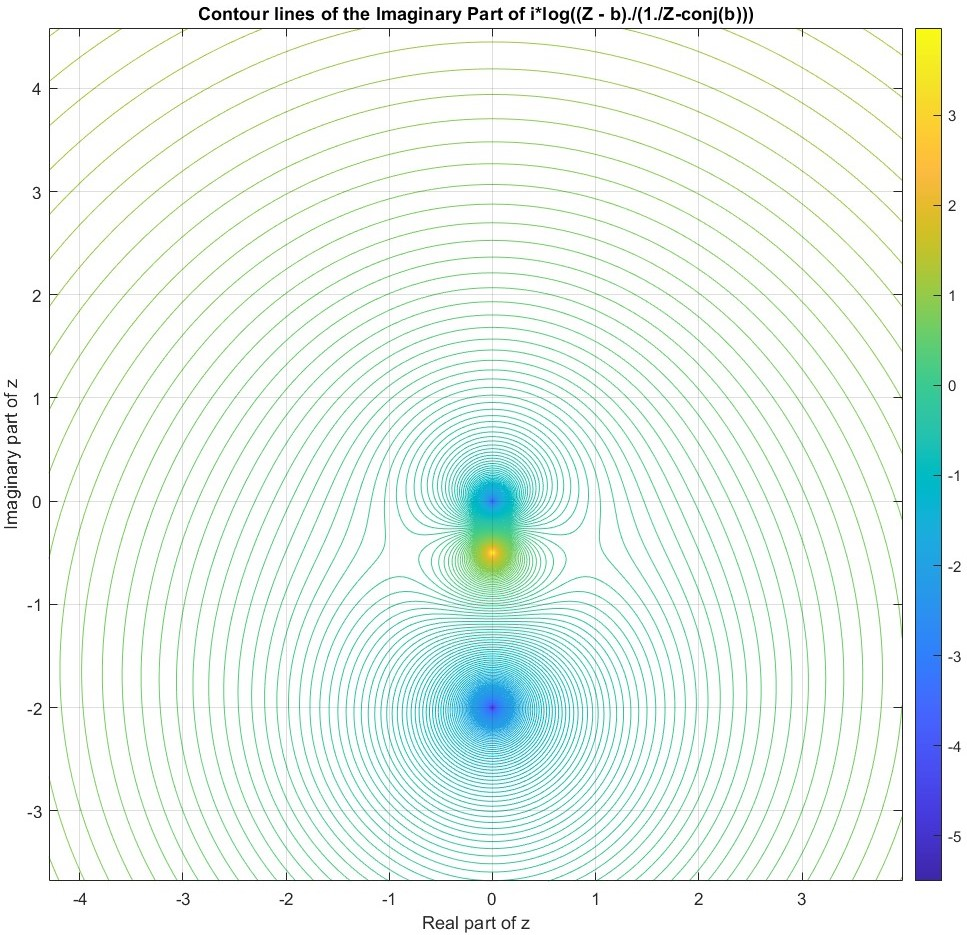
\includegraphics[width=1.\linewidth]{Figs/equal-pot, disk and charge, far view.jpg}
    \caption{\small The equipoentials from above. $y=0$ is the boundary between the dielectric and air. The three charges are the source charge at $(0, -2)$, and the two induced charge inside the disc. One at the origin, with the same sign of the source charge, and one differ. The equipoential of the disck is roughly visible.}
    \label{fig:enter-label}
\end{figure}

For the voltage below, start from charges (of different magintudes) in $W_+$, we need to determine the position and proportion the induced charge to meet the boundary conditions.

After some manipulation and trials, we derived that, the induced charge must be locate at $\overline{\zeta}_0$ above the disc. Previously, we found the structure with $q_t$ at $\overline{\zeta}_0$,  $q_b$, $q_r$ at ${\zeta}_0$ satisfies the conditions. Hence for the two charge at $\zeta_0$, and $1/\overline{\zeta_0}$, the corresponding charges must replicate the structure. Additionally, the charges at the origin do not affect surface charge distribution or the continuity of the voltage. 

\begin{figure}[H]
    \centering
    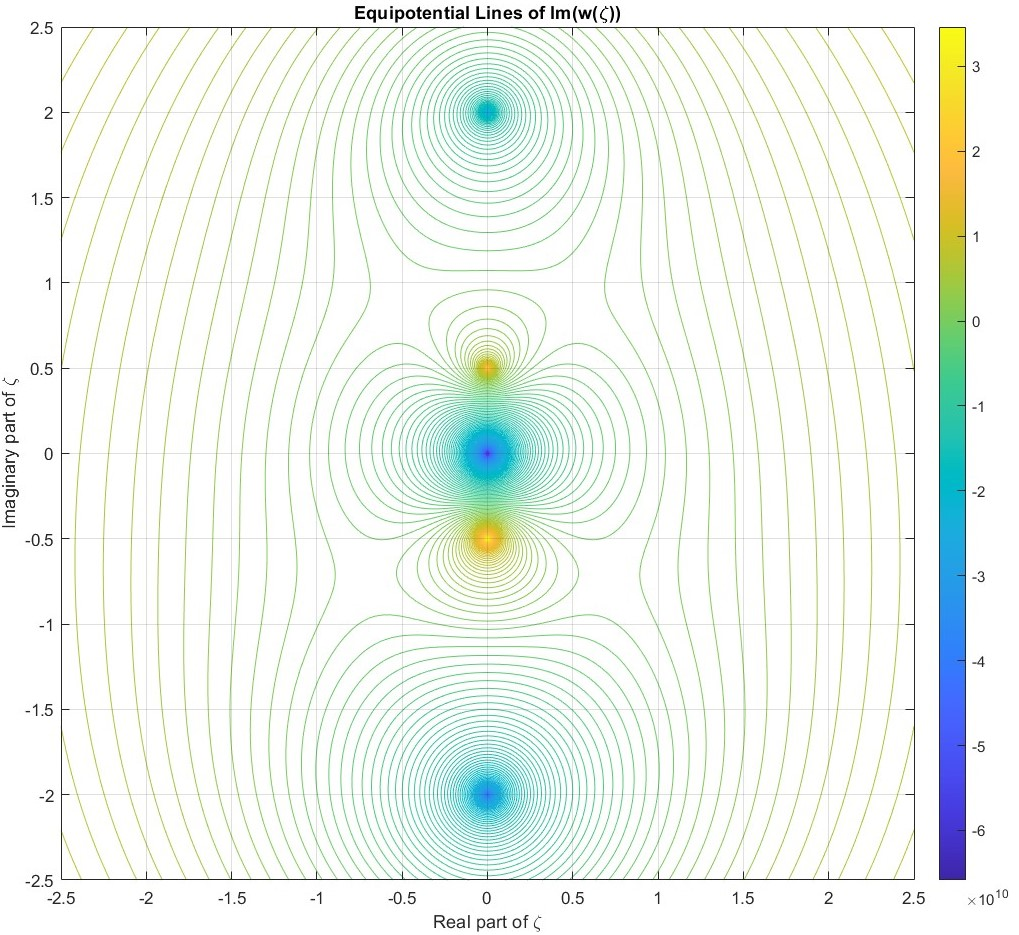
\includegraphics[width=1.\linewidth]{Figs/disc phase, inside dieletric.jpg}
    \caption{The equipotential from below. the potential contains six point charges, three of magnitude $q_b$ located separately at the source charge position, inside the semi-circle below, and the origin. Three of the fractions of the source charge $q_r$ are located symmetrically about the $y$-axis. Thus, there are two charges at the origin.}
    \label{fig:w_down}
\end{figure}


The complex potential of the dielectric area below $y=0$, of Figure (\ref{fig:w_down}) is \vspace{-.5em}
\begin{equation}\label{eqn:w_down}
    w_{-}(\zeta) = \frac{q}{2\pi \epsilon_0\epsilon_r} \im \left[ \log(\zeta - \zeta_0) - \log\left(\frac{1}{\zeta} - \overline{\zeta_0}\right) \right]
+\frac{q}{2\pi \epsilon_0\epsilon_r}\frac{\epsilon_r-1}{\epsilon_r+1}\im \left[ \log(\zeta - \overline{\zeta_0}) - \log\left(\frac{1}{\zeta} - \zeta_0\right) \right]    
\end{equation}
We check the voltage continuity at $y=0$, the other boundary conditions are satisfied simultaneously. From equation (\ref{eqn:w_up}) and equation (\ref{eqn:w_down}), \vspace{-1.em}
\[
V_+= \frac{q}{\pi \epsilon_0}\frac{1}{\epsilon_r+1} \left\{ \log\left(\sqrt{x^2+d^2}\right) -\log\left|\frac{1-\zeta\overline{\zeta_0}}{x}\right| \right\}
\]
\[
V_-= \frac{q}{2\pi \epsilon_0\epsilon_r} \left\{ \log\left(\sqrt{x^2+d^2}\right) -\log\left|\frac{1-\zeta\overline{\zeta_0}}{x}\right| \right\}
+\frac{q}{2\pi \epsilon_0\epsilon_r}\frac{\epsilon_r-1}{\epsilon_r+1} \left\{\log(\sqrt{x^2+d^2}) - \log\left|\frac{1-\zeta\zeta_0}{x}\right| \right\}
\]
We see that the three $\{...\}\coloneqq\alpha$ are equal on the $x-$axis, hence  \vspace{-1.em}
\[
V+=\frac{q}{\pi \epsilon_0}\frac{1}{\epsilon_r+1} \alpha\]
\[
V_-=\left(\frac{q}{2\pi \epsilon_0\epsilon_r} +\frac{q}{2\pi \epsilon_0\epsilon_r}\frac{\epsilon_r-1}{\epsilon_r+1}\right)\alpha
=\frac{q}{2\pi \epsilon_0\epsilon_r}\left( 1+\frac{\epsilon_r-1}{\epsilon_r+1}\right)\alpha
=\frac{q}{2\pi \epsilon_0\epsilon_r}\frac{2\epsilon_r}{\epsilon_r+1}\alpha=V_+
\]

\subsection{Mapping the Complex Potential to the $z$-plane}\label{cpt:slit_pot}
Next, we find a mapping $\zeta(z)$ from the semi-circle above to the slit, as Figure \ref{fig:map above} shows. The desired complex potential on the $z$-plane would be $w(\zeta(z))$.\vspace{-0.5em}
\begin{figure}[H]
    \centering
\adjustbox{frame=0.25pt,frame,margin=0.15,color=mycolor}{
    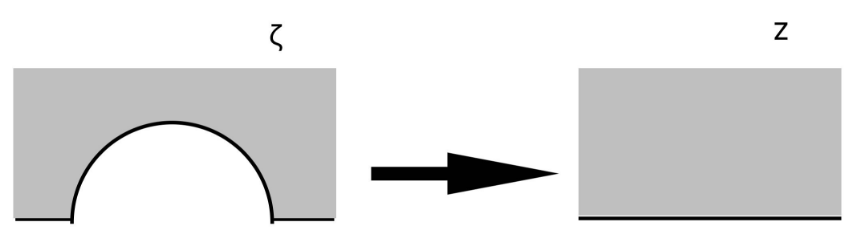
\includegraphics[width=1.\linewidth]{Figs/slit map brief.png}}
    \caption{\small The Mapping to addressing the charge, dielectric and slit problem. the shaded area represents the air and the upper arc of the disc, corresponding to the upper edge of the slit.}
    \label{fig:map above}
\end{figure}
\vspace{-0.5em}
In Matlab, $\zeta=z-\sqrt{z^2-1}
$ maps the left half of $\zeta$ plane, except the unit disc, to the left half of $z$ plane, and $\zeta=z+\sqrt{z^2-1}$ maps the right half of the $\zeta$ plane, except for the unit disc, to the right half of $z$ plane. Following the setting in Matlab, the complex potential on the $z$-plane is therefore divided into four parts.

Figure \ref{fig:vz above} is the equipotential of the voltage in the region $y>0$, on the $z$-plane\footnote{The $w(r<1)$ region must be excluded in the mapping. For an incorrect example see Appendix \ref{fig:wrong pot}.}. 

\begin{figure}[H]
    \centering
    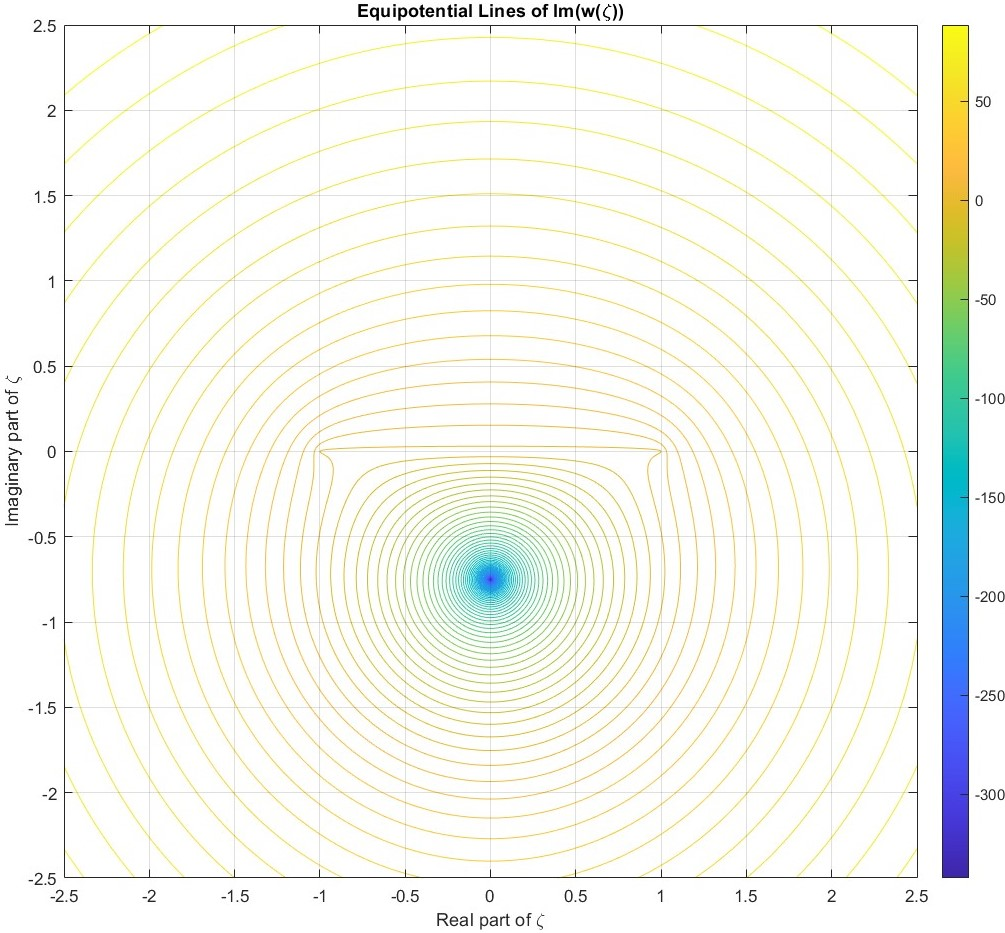
\includegraphics[width=1.\linewidth]{Figs/slit, Pot out dielectric, right.jpg}
    \caption{\small The equipotential lines of the area $y>0$, the 1, 2 quadrants. The dielectric is located in the region $y<0$. The slit is at $(x\in\pm1,y=0)$, and there is one equipotential intersect the slit. This is analogous  to streamline of a vortex under the slit of fluid dynamic. The source charge is at the centre of the concentric circles inside the dielectric.}
    \label{fig:vz above}
\end{figure}
For the complex potential above on the $z$-plane, start from equation (\ref{eqn:w_up}), leave $\zeta_0$ unchanged, use $\zeta(z)$ replacing $\zeta$ to rewrite $w(\zeta)$. In the first quadrant $(x>0, y>0)$, the complex potential is\vspace{-0.5em}
\[
\prescript{1}{}{w_{+}(z)} =\frac{q}{\pi\epsilon_0\epsilon_r}  \im \left[\log\left(z+\sqrt{z^2-1} - \zeta_0\right) - \log\left(\frac{1}{z+\sqrt{z^2-1}} - \overline{\zeta_0}\right)\right] \vspace{-0.5em}
\]
and in the second quadrant$(x<0, y>0)$, \vspace{-0.5em}
\[
\prescript{2}{}{w_{+}(z)} = \im \left[\log\left(z-\sqrt{z^2-1} - \zeta_0\right) - \log\left(\frac{1}{z-\sqrt{z^2-1}} - \overline{\zeta_0}\right)\right] \vspace{-2.em}
\]
    \begin{figure}[H]
        \centering
        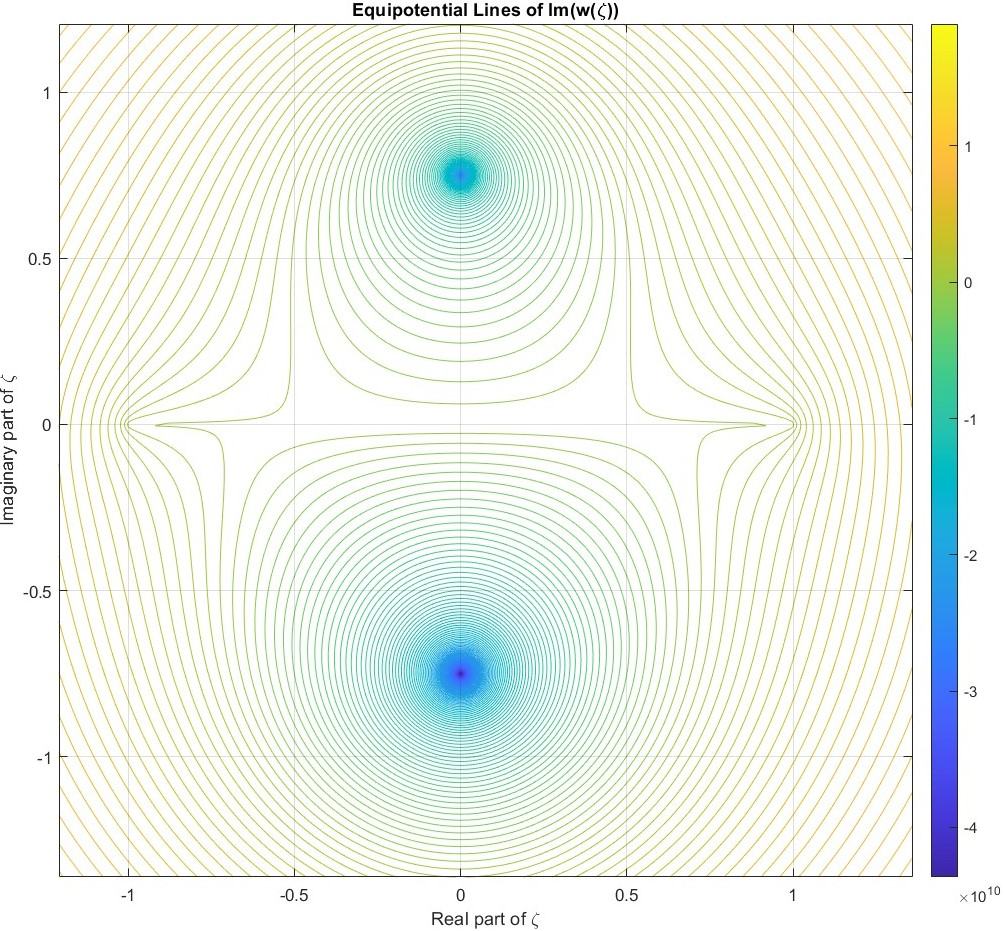
\includegraphics[width=1.\linewidth]{Figs/disc phase, inside dieletric, maped.jpg}
        \caption{\small The equipotentials in the region $y<0$, the 3, 4 quadrants. There is an induced charge above the dielectric. The slit is at $(x\in\pm1,y=0)$. One equipotential line reaches the slit, and the dense lines around the two cusps resemble the flow past a slit in fluid dynamics.}
        \label{fig:enter-label}
    \end{figure}\vspace{-1.em}
In the third quadrant$(x<0,y<0)$ and the fourth quadrant$(x>0,y<0)$, by equation (\ref{eqn:w_down}), we find the complex potentials are\vspace{-0.5em}:
\begin{align*}
\prescript{3}{}{w_{-}(z)} &= \frac{q}{2\pi \epsilon_0\epsilon_r} \im \left[ \log(z-\sqrt{z^2-1} - \zeta_0) - \log\left(\frac{1}{z-\sqrt{z^2-1}} - \overline{\zeta_0}\right) \right]\\
&+\frac{q}{2\pi \epsilon_0\epsilon_r}\frac{\epsilon_r-1}{\epsilon_r+1}\im \left[ \log(z-\sqrt{z^2-1} - \overline{\zeta_0}) - \log\left(\frac{1}{z-\sqrt{z^2-1}} - \zeta_0\right) \right]\vspace{-2.em}
\end{align*}
\begin{align*}
\prescript{4}{}{w_{-}(z)} &= \frac{q}{2\pi \epsilon_0\epsilon_r} \im \left[ \log(z+\sqrt{z^2-1} - \zeta_0) - \log\left(\frac{1}{z+\sqrt{z^2-1}} - \overline{\zeta_0}\right) \right]\\
&+\frac{q}{2\pi \epsilon_0\epsilon_r}\frac{\epsilon_r-1}{\epsilon_r+1}\im \left[ \log(z+\sqrt{z^2-1} - \overline{\zeta_0}) - \log\left(\frac{1}{z+\sqrt{z^2-1}} - \zeta_0\right) \right]\vspace{-0.5em}
\end{align*}
Combining the four parts we have the voltage across the entire $z$ plane, and the equipotentials.
    \begin{figure}[H]
        \centering
        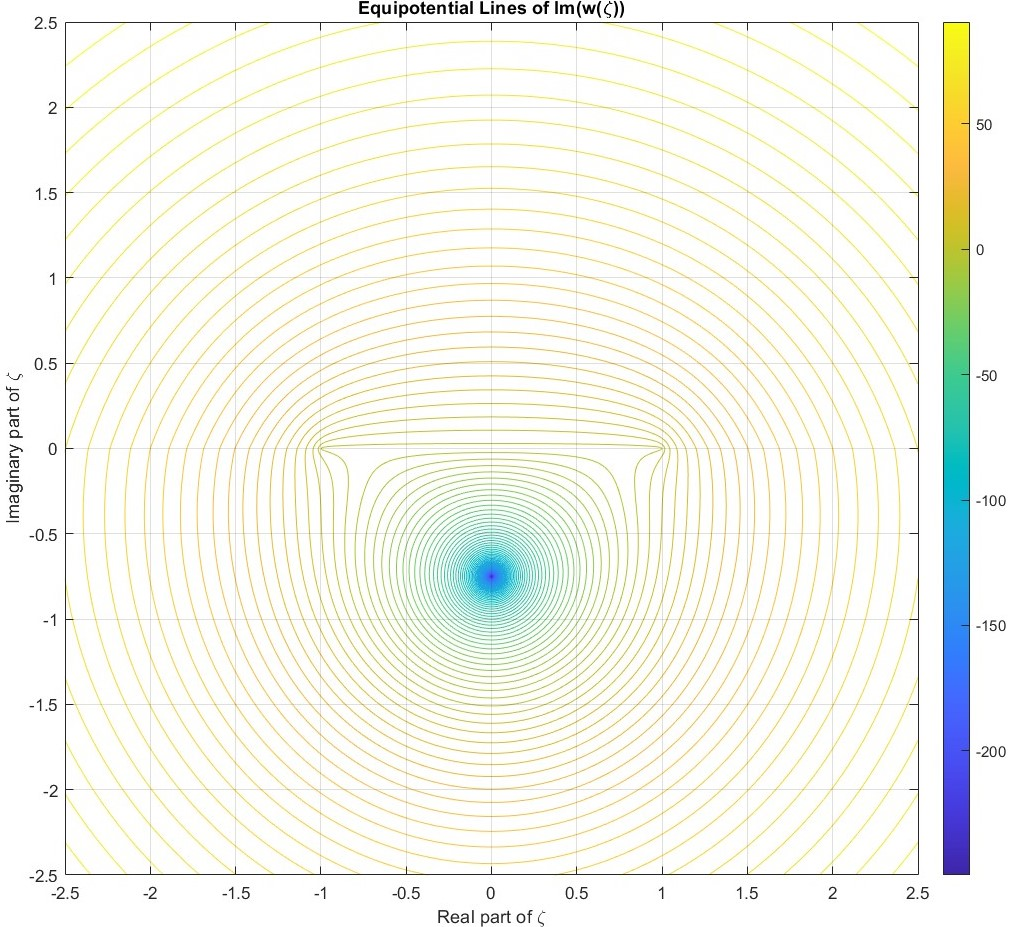
\includegraphics[width=1.\linewidth]{Figs/whole slit vot.jpg}
        \caption{\small The equipotentials of the entire plane are a combination of four parts. The slit is at $(\pm1,y=0)$. The induced charge is not seen. There is a slight distortion of voltages at $y=0$, the boundary between the dielectric and the region above.}
        \label{fig:enter-label}
    \end{figure}
 


\section{Summary}
    \hspace{0em}\indent This chapter discusses the boundary conditions for the electrodes, dielectric, and droplet problem, scaling it down to a thin film problem and further simplifying it to solve the Laplace and Poisson equations for the point charge and disc embedded in a dielectric. Subsequently, two models are established: one for the charged disc embedded in a dielectric and the another for a point charge embedded in a dielectric. 
    
    The shielding effect of the dielectric is derived, and conformal mapping methods are used to analyse the induced charge positions in a dielectric with specific symmetry. Based on these models and the conformal mapping technique, the complex potential for the charge, dielectric, and conductive slit is obtained, which also describes a distant conducting droplet in a point charge's electric field.
    
    In the process, complex analysis tools simplify the boundary conditions and the calculations of the electric field, aiding in the identification of induced charges. Whereas, when a dielectric is present, Gauss's Law at the dielectric boundary requires the use of electric field equations to determine the magnitude of the charge.

\pagebreak
\chapter{boundary line}

\section{derive surface charge density}
\[
z=\frac{\zeta}{2}+\frac{1}{2\zeta}
\]

\begin{align*}
 \sigma(z) &= \left| \frac{dw}{dz} \right| = \left| \frac{dw}{\df\zeta} \frac{\df \zeta}{\df z} \right| \\
\frac{\df\zeta}{\df z} &= \left( \frac{\df z}{\df\zeta} \right)^{-1}, \quad \frac{\df z}{\df\zeta} = \frac{1}{2} \left( 1 - \frac{1}{\zeta^2} \right) \\
\left. 1 - \frac{1}{\zeta^2} \right|_{\zeta=e^{\im \theta}} &= \left| \frac{\zeta^2 - 1}{\zeta^2} \right| = \left| \frac{e^{i2\theta} - 1}{e^{i2\theta}} \right| \\
\left| \frac{\df z}{\df\zeta} \right| &= \frac{1}{2} \left| e^{i2\theta} - 1 \right| = \frac{1}{2} \sqrt{(\cos 2\theta - 1)^2 + \sin^2 2\theta} \\
&= \frac{1}{2} \sqrt{\cos^2 2\theta + \sin^2 2\theta + 1 - 2\cos 2\theta} \\
&= \frac{1}{2} \sqrt{2 - 2\cos 2\theta} = \frac{\sqrt{2}}{2} \sqrt{1 - \cos 2\theta} \\
&= \frac{\sqrt{2}}{2} \sqrt{2\sin^2 \theta} = \sin \theta \\
\left| \frac{\df \zeta}{\df z} \right| &= \frac{1}{\sin \theta}
\end{align*}

\[
w(\zeta) = \frac{q_t}{2\pi \epsilon_0} \im \left[ \log(\zeta - \zeta_0) - i \log\left(\frac{1}{\zeta} - \overline{\zeta_0}\right) \right]
\]
define $\frac{q_t}{2\pi \epsilon_0}\im\coloneqq 1$
\[
\frac{dw}{d\zeta} \sim  \frac{1}{\zeta - \zeta_0} - \frac{1}{\frac{1}{\zeta} - \overline{\zeta_0}} \cdot \frac{-1}{\zeta^2} 
\]

\[
=  \frac{1}{\zeta - \zeta_0} + \frac{1}{\zeta + \zeta^2\overline{\zeta_0}} 
\]

\[
\text{at } \zeta = e^{i\theta}, \quad z = \frac{\zeta + \frac{1}{\zeta}}{2} = \cos \theta =x
\]
$\theta\in(0,\pi)$ and $x\in(1,-1)$ 
\[
\Rightarrow \sigma(\theta) = \left| \frac{dw}{d\zeta} \frac{d\zeta}{dz} \right| (\theta)= \frac{q_t}{2\pi \epsilon_0}\left| \frac{1}{e^{i\theta} - \zeta_0} + \frac{1}{e^{i\theta} + e^{i2\theta}\overline{\cdot \zeta_0}} \right| \cdot \frac{1}{\sin \theta}
\]
in $x$, and $y\equiv0$
\[
\Rightarrow \sigma(x) = \frac{q_t}{2\pi \epsilon_0}\left| \frac{1}{x+\im\sqrt{1-x^2} - \zeta_0} + \frac{1}{x+\im\sqrt{1-x^2} + (x+\im\sqrt{1-x^2})^2\overline{\cdot \zeta_0}} \right| \cdot \frac{1}{\sqrt{1-x^2}}
\]




\section{$h$}
$w(z)$ $w_1$,$w_2$\\
$w_1$
\[
w = i \log \left( z + \sqrt{z^2 - 1} - \zeta_0 \right) - i \log \left( \frac{1}{z + \sqrt{z^2 - 1}} - \overline{\zeta_0} \right)
\]
\[
\frac{\partial w_1}{\partial z} = \frac{1}{z + \sqrt{z^2 - 1} - \zeta_0} \cdot \left( 1 + \frac{z}{\sqrt{z^2 - 1}} \right)
\]
\[
= \frac{1}{\sqrt{z^2 - 1}} \cdot \frac{z + \sqrt{z^2 - 1}}{z + \sqrt{z^2 - 1} - \zeta_0}
\]
\( z = x \), \( x \in (0,1) \), $\zeta_0\coloneqq-a\im$
\[
\frac{\partial w_1}{\partial z} \Bigg|_{z=x} = \frac{1}{\im\sqrt{1 - x^2}} \cdot \frac{x + i \sqrt{1 - x^2}}{x + i \left( a + \sqrt{1 - x^2} \right)}
\]
\[
\left| \frac{\partial w_1}{\partial z} \right|_{z=x}= \frac{1}{\sqrt{1 - x^2}} \cdot \frac{\left|x + i \sqrt{1 - x^2}\right|}{\sqrt{x^2 + a^2 + \left( \sqrt{1 - x^2} \right)^2 + 2a \sqrt{1 - x^2}}}
\]

\[
\left| \frac{\partial w_1}{\partial z} \right|_{z=x} = \frac{1}{\sqrt{1 - x^2}} \cdot \frac{1}{a^2 + 1 + 2a \sqrt{1 - x^2}}
\]
as
\[
a^2 + 1 + 2a \sqrt{1 - x^2}>a^2 + 1 + 2a=(a+1)^2\geq 0
\]
$w_2$\\
\[
\frac{\partial w_2}{\partial z} = -i \cdot \frac{1}{\frac{1}{z + \sqrt{z^2 - 1}} - \overline{\zeta_0}} \cdot \left(\frac{1}{z+\sqrt{z^2 - 1}}\right)'
\]
\[= -i \cdot \frac{z + \sqrt{z^2 - 1}}{1 - \overline{\zeta_0}\left(z + \sqrt{z^2 - 1}\right)} \cdot \frac{-1}{\left(z+\sqrt{z^2 - 1}\right)^2} \cdot \left( 1 + \frac{z}{\sqrt{z^2 - 1}} \right)
\]
\[
= \frac{i}{\sqrt{z^2 - 1}} \cdot \frac{z + \sqrt{z^2 - 1}}{1 - a i \left( z + \sqrt{z^2 - 1} \right)}
\]
 \( z = x \)
\[
\frac{\partial w_2}{\partial z} \Bigg|_{z=x} = \frac{\im}{\im\sqrt{1 - x^2}} \cdot \frac{1}{1 - a i x - a \im\im \sqrt{1 - x^2}}
\]

\[
\left| \frac{\partial w_2}{\partial z} \right|_{z=x}= \frac{1}{\sqrt{1 - x^2}} \cdot \frac{1}{\sqrt{(1 + a \sqrt{1 - x^2})^2 + (a x)^2}}
\]

\[
\left| \frac{\partial w_2}{\partial z} \right|_{z=x} = \frac{1}{\sqrt{1 - x^2}} \cdot \frac{1}{1 + a^2 + 2 a \sqrt{1 - x^2}}
\]
hence
\[
\left|\frac{\df w}{\df z}\right|_{z=x}=\left|\frac{\df w_1}{\df z}+\frac{\df w_2}{\df z}\right|_{z=x} = \frac{2}{\sqrt{1 - x^2}} \cdot \frac{1}{1 + a^2 + 2 a \sqrt{1 - x^2}}
\]
that is, in $z$, the charge density on the upper slit
\[
\sigma\sim \frac{2}{\sqrt{1 - x^2}} \cdot \frac{1}{1 + a^2 + 2 a \sqrt{1 - x^2}}
\]
\begin{figure}[H]
    \centering
    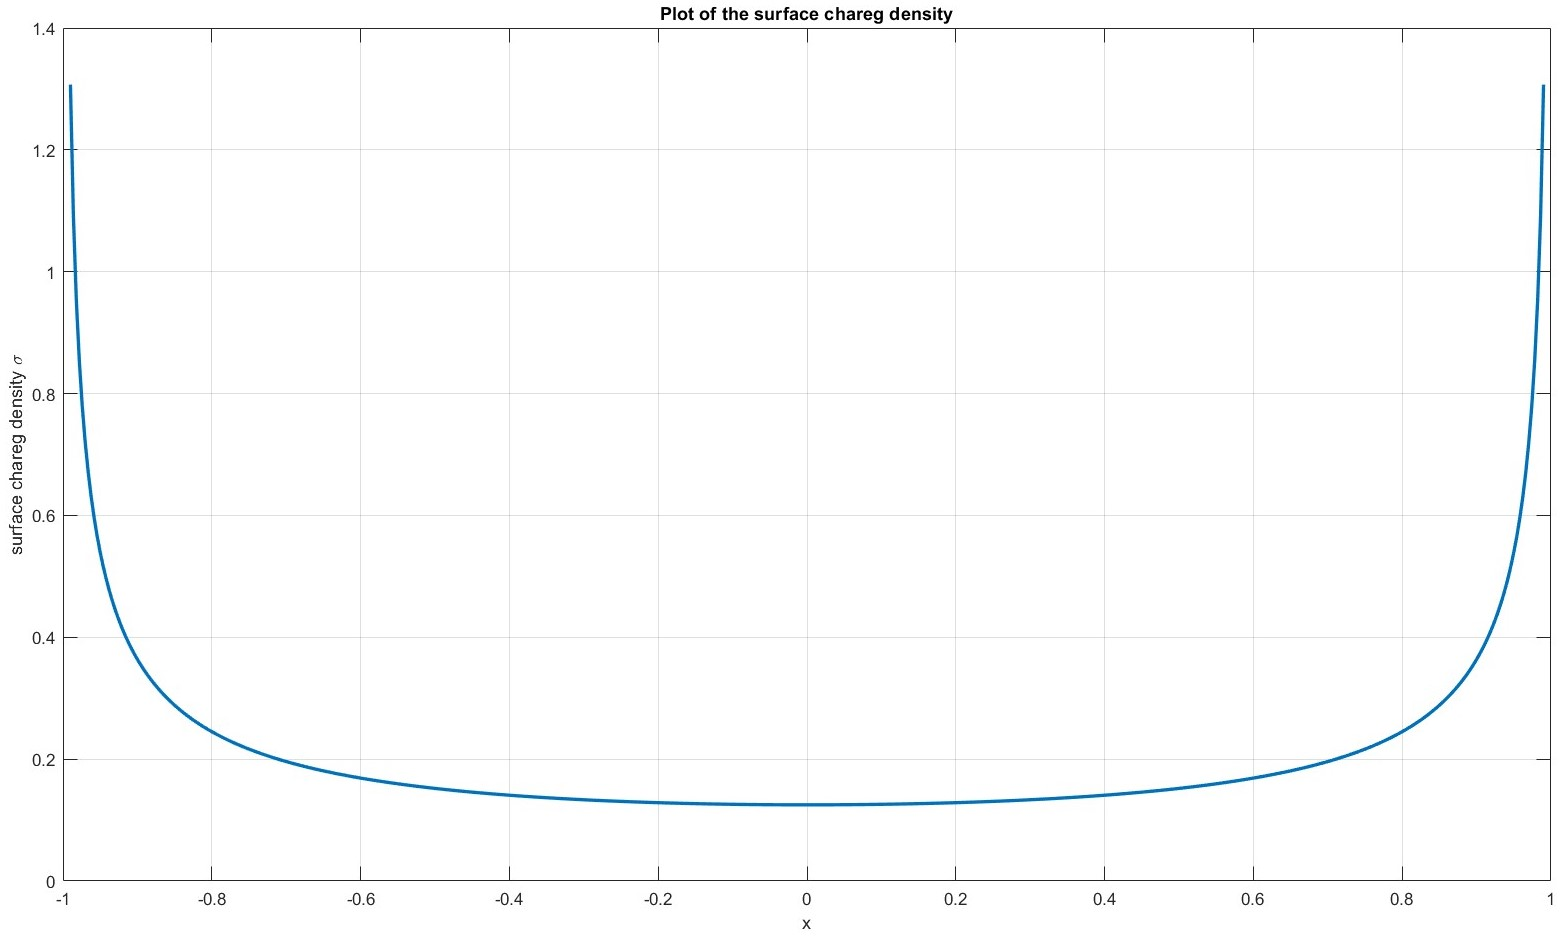
\includegraphics[width=0.85\linewidth]{Figs/surface charge density.jpg}
    \caption{\small surface charge density, $x\in(-0.99, 0.99)$, at the boundary area, the value goes to $\infty$, hence omitted}
    \label{fig:enter-label}
\end{figure}
and
\[
\int \sigma \sim \arctan \sqrt{1-x^2}
\]
\pagebreak

\chapter{Conclusion}
\hspace{0em}\indent The study employs a method that combines modelling and conformal mapping to derive the complex potential, the surface curve, and the surface charge density, of charged droplets. By omitting the detailed local geometry, this approach simplifies the physical problem, allowing for a more tractable and generalizable droplet curve solution. The results are consistent with experimental observations, supporting the method's validity to a sufficiently accurate scale. 

However, the limitations of the method must also be acknowledged. In the local contact angle region, the current mapping function proves inadequate, and the global complex potential function fails to accurately capture the local contact angle.

\vspace{1em}\\
\noindent \textbf{Key findings include}:
\begin{itemize}
    \item The boundary functions of charged droplets are derived via multiple methods, revealing that the Crowdy map contains analytical solutions for the $90\degree$ contact angle charged droplets on a conducting substrate, where an induced charge is located above the droplet.

    \item Complex potential for the charge, dielectric, and $0\degree$ contact angle droplet model were derived. Conformal mapping techniques were used to study the corresponding thin-film models and positions of induced charges in a dielectric with specific symmetry. The shielding effect of the dielectric was analysed. 

    \item The local droplet height function, based on the surface charge density, is formulated from the complex potential function. The droplet curves for two scenarios were derived, and the surface charge density and droplet curves show agreement with physical and numerical studies.

\end{itemize}

\noindent\textbf{Future Work}
\begin{itemize}
    \item The electrical, mechanical, and fluid properties near the contact angle are more likely local experimental or numerical issues. Achieving a complex potential function that is applicable both globally and locally through conformal mapping presents significant challenges. Therefore, the contact angle should be treated as an exogenous, experimentally determined physical property. Methods such as the generalised Joukowski transformation can then be employed to adjust the mapping's contact angle based on observed values, with the aim of obtaining more precise surface functions for analysing potential variations at the contact angle.


    \item Develop more accurate models for charged droplets controlled by electrodes to optimise the analytical functions. Although the solutions obtained in this study align with experimental observations, the effectiveness of the models has not been directly addressed. Further validation could include exploring whether the dielectric and disc model in a uniform electric field offers a better representation of the droplet surface and complex potential functions, and identifying other charge distribution models that sufficiently account for cases involving electrodes.

\end{itemize}

%The complex potential formed by the charged droplet on a conducting plate, as observed in the conformal mapping study, approximates ellipses with one focus coinciding at a distance, which might have connections to models of galaxy rotation, among others. In fluid dynamics, this phenomenon seems to resemble vortices formed above a depression on the riverbed, which could be explored in future research.


\pagebreak

\pagebreak
\addcontentsline{toc}{chapter}{References}

%\renewcommand\bibname{{References}}
\bibliography{References}
\bibliographystyle{apalike}

\appendix

\chapter{derivations}

\section{from minimal energy equation to the variation}

\indent These two derivations are not completed, they are recorded here briefly for further investigation.\\
\indent Start with conducting fluid droplet $\Omega\in\mathbb{R}^2$ surrounds as usual
\[\mathcal{E} = \gamma \mathcal{P} - \frac{\epsilon}{2} \int_{R^2 \setminus \Omega} |E|^2 \, dS\hspace{0.5em},\hspace{1em}\mathcal{E}_e\coloneqq- \frac{\epsilon}{2} \int_{R^2 \setminus \Omega} |E|^2 \, dS\]
\indent For the minimal energy, a small variation $\delta\Omega$ leads to no change in energy, $\delta\mathcal{E}=0$.\\
\indent The variation in the surface tension is:
\[\delta (\gamma\mathcal{P})=\gamma\delta\mathcal{P}\hspace{0.5em},\hspace{1em}\delta\mathcal{P}=\int_{\partial \Omega}\kappa\df l\]
\indent On the other hand, since all the charges are distributed on the boundary of the area $R^2 \setminus \Omega$, assume $\mathcal{E}_e|_{r\rightarrow\infty}\sim O(\frac{1}{r})\sim 0$ and $\mathcal{E}_e|_{\partial \Omega}=\frac{\lambda}{\epsilon}$,
\[
\mathcal{E}_e=-\frac{\epsilon}{2}\int_{\mathbb{R}^2\setminus \Omega}|E|^2\df S=-\frac{\epsilon}{2}\int_{\partial \Omega}|\frac{\lambda}{\epsilon}|^2\df l+ other \longrightarrow\delta \mathcal{E}_e \approx-\frac{\lambda^2}{2\epsilon}\int_{\partial \Omega}\df l
\]
Although the contribution of the boundary to $E_e$ is acounted for, the area may affect $E_e$, which is not rigorously excluded.\\
\indent Try the divergence theorem, The variation in the electric field $\delta E_e$ is:
\begin{equation*}
    \delta \mathcal{E}_e=\delta\left(-\frac{\epsilon}{2}\int_{\mathbb{R}^2\setminus\Omega}|E|^2 \df S
\right)=-\frac{\epsilon}{2}\int_{\mathbb{R}^2\setminus\Omega}\delta|E|^2 \df S=-\frac{\epsilon}{2}\int_{\mathbb{R}^2\setminus\Omega}2\mathbf{E}\cdot\delta\mathbf{E} \df S
\end{equation*}
\indent Let $\mathbf{G}\coloneqq\mathbf{E}\delta V$
\begin{equation*}
    \begin{split}
    \delta \mathcal{E}_e&=-\epsilon\int_{\mathbb{R}^2\setminus\Omega}\mathbf{E}\cdot\delta(-\nabla V) \df S=\epsilon\int_{\mathbb{R}^2\setminus\Omega}\mathbf{E}\cdot(\nabla \delta V) \df S\\
\text{use } \nabla\cdot(\mathbf{A}\phi)=\phi\nabla\cdot\mathbf{A}+\mathbf{A}\cdot\nabla\phi\\
    &=\epsilon\int_{\mathbb{R}^2\setminus\Omega}\nabla\cdot(\mathbf{E}\, \delta V) -\delta V \eqnmarkbox[black]{node1}{\nabla\cdot\mathbf{E}}\df S\\
    &=\epsilon\int_{\mathbb{R}^2\setminus\Omega}\nabla\cdot(\mathbf{E}\, \delta V) \df S \xlongequal[ ]{\text{div thm}}\oint_{...}\mathbf{G}\cdot\hat{\mathbf{n}}\df l=\int_{\partial \Omega}...+\eqnmarkbox[black]{node2}{\int_{r\rightarrow\infty}\mathbf{E}}\cdot\hat{\mathbf{n}}\, \delta V\df l\\
    &=\epsilon\int_{\partial\Omega}\mathbf{E}\cdot\hat{\mathbf{n}}\, \delta V \df l\\
\text{Since }\mathbf{E}|_{\partial \Omega}=\frac{\lambda}{\epsilon}\hat{\mathbf{n}}\\
    \delta \mathcal{E}_e&=\lambda\int_{\partial \Omega}\delta V \df l
    \end{split}
\end{equation*}
\annotate[yshift=1em]{above, right, label above}{node1}{$\nabla \cdot \mathbf{E}|_{\mathbb{R}^2\setminus \Omega}= 0$}
\annotate[yshift=1em]{above, right, label above}{node2}{$=0,\mathbf{E}|_{r\rightarrow\infty}\rightarrow 0$}
\indent In order to have the desired result, we would expect\footnote{Expect to refer to \cite{Griffiths_2017}, pp. 103, to figure out why $\delta V$ is this. As only the outside of the droplet has $\mathbf{E}/neq 0$, there is a $\frac{1}{2}$}
\[\int_{\partial \Omega} \delta V \df l =-\frac{\lambda}{2\epsilon}\int_{\partial \Omega}\df l\longrightarrow\delta V = -\frac{\lambda}{2\epsilon}\]
\indent dig more
\[\delta V =  \frac{1}{2}(\mathbf{E_{above}}+\eqnmarkbox[black]{node1}{{\mathbf{E}_{below}}})\cdot \delta \mathbf{d}=\frac{\mathbf{E_{above}}}{2}\delta \mathbf{d}=\frac{\lambda}{2\epsilon}\hat{\mathbf{n}}\cdot \delta \mathbf{d}\]
\annotate[yshift=1em]{above, right, label above}{node1}{$=0$}
Assume $\mathbf{d}=\hat{\mathbf{n}}$. Still problematic though, sign and others, later.
%\subsection{First Subsection Title}

%a1c2
%\section{First Section Title}

%a1c3
\section{potentials with boundary conditions}
\[w=\log (z -b) + \log (z-\frac{a^2}{b})-\log(z)\Longrightarrow w =\log (z +\frac{a^2}{z}-b-\frac{a^2}{b})\]
this function\footnote{Refering to Fluid Dynamic 1 exam paper year 2014 question 4.} is a combination of one source at $b$, another one at $\frac{a^2}{b}$, and a sink at $0$.

on $z=a e^{\mathrm{i}  \theta}$
\[ w=\log (2 a \cos{\theta}-b-\frac{a^2}{b})\]
hence
\[\Im[w]= 0 \text{ or } -\pi\]

\pagebreak
%\renewcommand\bibname{{References}}
%\bibliography{References}
%\bibliographystyle{plain}
\chapter{Mathematical Considerations to Note}

\section{Complx}
\subsection{Basis}

\begin{equation*}
\begin{split}
z = x + iy, \quad \overline{z} = x - iy \Longrightarrow &x = \frac{z + \overline{z}}{2}, \quad y = \frac{z - \overline{z}}{2i} \\
\Longrightarrow &\frac{\partial z}{\partial x} = 1, \quad \frac{\partial \overline{z}}{\partial x} = 1, \quad \frac{\partial z}{\partial y} = i, \quad \frac{\partial \overline{z}}{\partial y} = -i \\
&\frac{\partial x}{\partial z} = \frac{1}{2}, \quad \frac{\partial x}{\partial \overline{z}} = \frac{1}{2}, \quad \frac{\partial y}{\partial z} = -\frac{i}{2}, \quad \frac{\partial y}{\partial \overline{z}} = \frac{i}{2}
\end{split}
\end{equation*}

\begin{prop}{$\frac{\partial z}{\partial x}$ and $\frac{\partial x}{\partial z}$}
\end{prop}
\[x=\frac{z+\overline{z}}{2}\Longrightarrow \left.\frac{\partial x}{\partial z}\right|_{\overline{z}}=\frac{1}{2}\]
\[z=x+\im y \Longrightarrow \left.\frac{\partial z}{\partial x}\right|_{y}=1\neq\frac{1}{\frac{\partial x}{\partial z}}\]

\begin{prop}{conjugate of derivative}
\end{prop}
\[\overline{\left(\frac{\df f}{\df z}\right)}=\frac{\df \overline{f}}{\df z}\]
\[\overline{\left(\frac{\df f}{\df z}\right)}\neq\frac{\df \overline{f}}{\df \overline{z}}\]

\section{Del Operators in Complex Form}
\subsection{Derivatives}

Using the chain rule:
\[ 
\frac{\partial}{\partial x} = \frac{\partial z}{\partial x} \frac{\partial}{\partial z} + \frac{\partial \overline{z}}{\partial x} \frac{\partial}{\partial \overline{z}} = \frac{\partial}{\partial z} + \frac{\partial}{\partial \overline{z}} 
\]
\[ 
\frac{\partial}{\partial y} = \frac{\partial z}{\partial y} \frac{\partial}{\partial z} + \frac{\partial \overline{z}}{\partial y} \frac{\partial}{\partial \overline{z}} = i \frac{\partial}{\partial z} - i \frac{\partial}{\partial \overline{z}} 
\]


\subsection{Gradient}
\[ 
\nabla \coloneqq\left(\frac{\partial}{\partial x}\,,\quad \frac{\partial}{\partial y}\right)= \left( \frac{\partial}{\partial z} + \frac{\partial}{\partial \overline{z}}\,, \quad i \left( \frac{\partial}{\partial z} - \frac{\partial}{\partial \overline{z}} \right) \right) 
\]

\subsection{Divergence}

\begin{equation*}
\begin{split}
\nabla \cdot \mathbf{F} &= \left( \frac{\partial}{\partial x} \mathbf{F}_x + \frac{\partial}{\partial y} \mathbf{F}_y \right) \\
&= \left( \frac{\partial}{\partial z} + \frac{\partial}{\partial \overline{z}} \right) \mathbf{F}_x + \left( i \frac{\partial}{\partial z} - i \frac{\partial}{\partial \overline{z}} \right) \mathbf{F}_y \\
&= \frac{\partial \mathbf{F}_x}{\partial z} + \frac{\partial \mathbf{F}_x}{\partial \overline{z}} + i \frac{\partial \mathbf{F}_y}{\partial z} - i \frac{\partial \mathbf{F}_y}{\partial \overline{z}}
\end{split}
\end{equation*}

\subsection{Laplacian}

\begin{equation*}
\begin{split}
\frac{\partial}{\partial x} \left( \frac{\partial}{\partial x} \right) &= \left( \frac{\partial}{\partial z} + \frac{\partial}{\partial \overline{z}} \right) \left( \frac{\partial}{\partial z} + \frac{\partial}{\partial \overline{z}} \right) \\
&= \frac{\partial^2}{\partial z^2} + \frac{\partial^2}{\partial z \partial \overline{z}} + \frac{\partial^2}{\partial \overline{z} \partial z} + \frac{\partial^2}{\partial \overline{z}^2} \\
&= \frac{\partial^2}{\partial z^2} + 2 \frac{\partial^2}{\partial z \partial \overline{z}} + \frac{\partial^2}{\partial \overline{z}^2}
\end{split}
\end{equation*}

\begin{equation*}
\begin{split}
\frac{\partial}{\partial y} \left( \frac{\partial}{\partial y} \right) &= \left( i \frac{\partial}{\partial z} - i \frac{\partial}{\partial \overline{z}} \right) \left( i \frac{\partial}{\partial z} - i \frac{\partial}{\partial \overline{z}} \right) \\
&= - \left( \frac{\partial^2}{\partial z^2} - \frac{\partial^2}{\partial z \partial \overline{z}} - \frac{\partial^2}{\partial \overline{z} \partial z} + \frac{\partial^2}{\partial \overline{z}^2} \right) \\
&= - \left( \frac{\partial^2}{\partial z^2} - 2 \frac{\partial^2}{\partial z \partial \overline{z}} + \frac{\partial^2}{\partial \overline{z}^2} \right)
\end{split}
\end{equation*}

Laplacian:
\begin{equation*}
\begin{split}
\nabla^2 &= \frac{\partial}{\partial x} \left( \frac{\partial}{\partial x} \right) + \frac{\partial}{\partial y} \left( \frac{\partial}{\partial y} \right) \\
&= \left( \frac{\partial^2}{\partial z^2} + 2 \frac{\partial^2}{\partial z \partial \overline{z}} + \frac{\partial^2}{\partial \overline{z}^2} \right) - \left( \frac{\partial^2}{\partial z^2} - 2 \frac{\partial^2}{\partial z \partial \overline{z}} + \frac{\partial^2}{\partial \overline{z}^2} \right) \\
&= 4 \frac{\partial^2}{\partial z \partial \overline{z}}
\end{split}
\end{equation*}

The general solution to the two-dimensional Laplace equation in complex variables \( z = x + iy \) and its conjugate \( \overline{z} = x - iy \) is:
\[
\nabla^2 \phi = 4 \frac{\partial^2 \phi}{\partial z \partial \overline{z}} = 0
\]
This implies that the potential \( \phi \) can be expressed as:
\[
\phi = w(z) + \overline{w(z)}
\]
where \( w(z) \) is an analytic function of \( z \) and \( \overline{w(z)} \) is its Schwarz conjugate.

\subsubsection{Complex Potential for a Charged Metal Disk}
\textbf{General Solution}
The potential \( V \) in the complex plane can be represented by an analytic function \( f(z) \):
\[
f(z) = \sum_{n=-\infty}^{\infty} c_n z^n
\]
\textbf{Special Case: Logarithmic Function}
For a charged metal disk, a specific solution is:
\[
f(z) = \frac{Q}{2\pi \epsilon_0} \log(z)
\]
where \( Q \) is the total charge and \( \epsilon_0 \) is the permittivity of free space.
\textbf{Justification}
\begin{itemize}
    \item \textbf{Analyticity}: \(\log(z)\) is analytic except at \( z = 0 \).
    \item \textbf{Boundary Conditions}: Fits potential on the unit disk boundary \( |z| = 1 \).
    \item \textbf{Physical Meaning}: Models potential around charged conductors.
\end{itemize}
\textbf{Relationship}
The logarithmic term fits within the general solution framework:
\[
f(z) = \sum_{n=1}^{\infty} a_n z^n + b_n z^{-n} + c_0 \log(z)
\]

\subsection{Cauchy Riemann Condition}

\begin{thm}{Cauchy Riemann Condition (f CRC= f hoarmonic)}
\end{thm}

\begin{center}
$f(z)=\phi+\im\psi$ analytic at $z_0\Longleftrightarrow$ CRC and $\psi,\phi\in \mathbb{R}$, $\psi,\phi\in C^1$\footnote{$C^1 \coloneqq$1st derivate cts.}
\end{center}
CRC:
\begin{align*}
    \partial_x \phi &=\partial_y \psi    \\
    \partial_x \psi &= -\partial_y \phi
\end{align*}

\begin{prop}{$\frac{\df f}{\df z}$ when CRC}
\end{prop}
\begin{equation*}
f CRC \Longrightarrow f_z=\partial_x \phi+ \im \partial_x \psi= \partial_y \psi\textcolor{red}{-}\im\partial_y \phi
\end{equation*}
on $\forall \mathbb{C}$, NOT only along $\hat{\mathbf{x}}$ or $\hat{\mathbf{y}}$ direction.


\subsection{Curvature in Complex form}
\subsection{Normalized Gradient in Complex Form}

The gradient $\nabla f$ in terms of $x$ and $y$ is given by:
\[ 
\nabla f = \left( \frac{\partial f}{\partial x}, \frac{\partial f}{\partial y} \right) 
\]
In terms of $z$ and $\overline{z}$, it is expressed as:
\[ 
\nabla f = \left( f_z + f_{\overline{z}}, \quad i \left( f_z - f_{\overline{z}} \right) \right) 
\]

The magnitude of the gradient $|\nabla f|$ is:
\[ 
\begin{split}
|\nabla f| &= \sqrt{\left( \frac{\partial f}{\partial x} \right)^2 + \left( \frac{\partial f}{\partial y} \right)^2} \\
&= \sqrt{\left( f_z + f_{\overline{z}} \right)^2 + \left( i \left( f_z - f_{\overline{z}} \right) \right)^2} \\
&= \sqrt{\left( f_z + f_{\overline{z}} \right)^2 - \left( f_z - f_{\overline{z}} \right)^2} \\
&= \sqrt{4 f_z f_{\overline{z}}}
\end{split}
\]

The normalized gradient $\frac{\nabla f}{|\nabla f|}$ is given by:
\[ 
\begin{split}
\frac{\nabla f}{|\nabla f|} &= \left( \frac{\frac{\partial f}{\partial x}}{|\nabla f|}, \frac{\frac{\partial f}{\partial y}}{|\nabla f|} \right) \\
&= \left( \frac{f_z + f_{\overline{z}}}{\sqrt{4 f_z f_{\overline{z}}}}, \quad \frac{i (f_z - f_{\overline{z}})}{\sqrt{4 f_z f_{\overline{z}}}} \right) \\
&= \frac{1}{2} \left( \frac{f_z + f_{\overline{z}}}{\sqrt{f_z f_{\overline{z}}}}, \quad \frac{i (f_z - f_{\overline{z}})}{\sqrt{f_z f_{\overline{z}}}} \right) \\
&= \frac{1}{2} \left( \sqrt{\frac{f_z}{f_{\overline{z}}}} + \sqrt{\frac{f_{\overline{z}}}{f_z}}, \quad i \left( \sqrt{\frac{f_z}{f_{\overline{z}}}} - \sqrt{\frac{f_{\overline{z}}}{f_z}} \right) \right)
\end{split}
\]

\begin{prop}
$f$ analytic $\Longrightarrow |\nabla f|=0\Longrightarrow$ Mean Curvature, $K\coloneqq \nabla\cdot\frac{\nabla f}{|\nabla f|}$ is undefined in $\mathbb{C}$.    
\end{prop}
\[f\text{ analytic }\Longrightarrow \frac{\partial f}{\partial \overline{z}} = 0\]
hence the gradient magnitude is:
\[ |\nabla f| = \sqrt{4 f_z f_{\overline{z}}} \xrightarrow[]{f_{\overline{z}} = 0}|\nabla f| = 0\]

This means \(|\nabla f|\) is zero, so the curvature is undefined. However, the function \( f \) can still be a curve.

\begin{eg}{Analytic Function, a curve}
\end{eg}
Consider the analytic function:
   \[ f(z) = z^2 = (x + iy)^2 = x^2 - y^2 + 2ixy \]
where
    \[ u(x, y) = x^2 - y^2, \quad v(x, y) = 2xy \]
Gradient:
   \[ \frac{\partial f}{\partial x} = 2x + 2iy \]
   \[ \frac{\partial f}{\partial y} = -2y + 2ix \]

Gradient magnitude:
   \[ |\nabla f| = \sqrt{\left( 2x + 2iy \right)^2 + \left( -2y + 2ix \right)^2} \]
as
   \[ \left( 2x + 2iy \right)^2 = 4x^2 - 4y^2 + 8ixy \]
   \[ \left( -2y + 2ix \right)^2 = 4y^2 - 4x^2 - 8ixy \]
find
   \[ |\nabla f| = \sqrt{4x^2 - 4y^2 + 8ixy + 4y^2 - 4x^2 - 8ixy} = \sqrt{0} = 0 \]
The gradient magnitude is zero, but the function \( f(z) = z^2 \) is a curve (a parabola).

\begin{prop}
    $\operatorname{Im}(f)=0$ and f analytic
\end{prop}
\[ \operatorname{Im}(f) \coloneqq 0 \Longrightarrow f = u(x, y) \]

f analytic, hence by Cauchy-Riemann equations:
\[ \frac{\partial u}{\partial x} = \frac{\partial v}{\partial y}=0, \quad \frac{\partial u}{\partial y} = -\frac{\partial v}{\partial x}=0 \Longrightarrow\frac{\partial u}{\partial x} = 0, \quad \frac{\partial u}{\partial y} = 0\]
Yet $u \not\equiv 0$, E.G. $f=-\im \log z$, on $|z|=1$, $\operatorname{Im}(f)=\log 1=0$, $\operatorname{Re}(f)=\theta\neq0$.
\section{mistakes}
\begin{figure}[H]
    \centering
    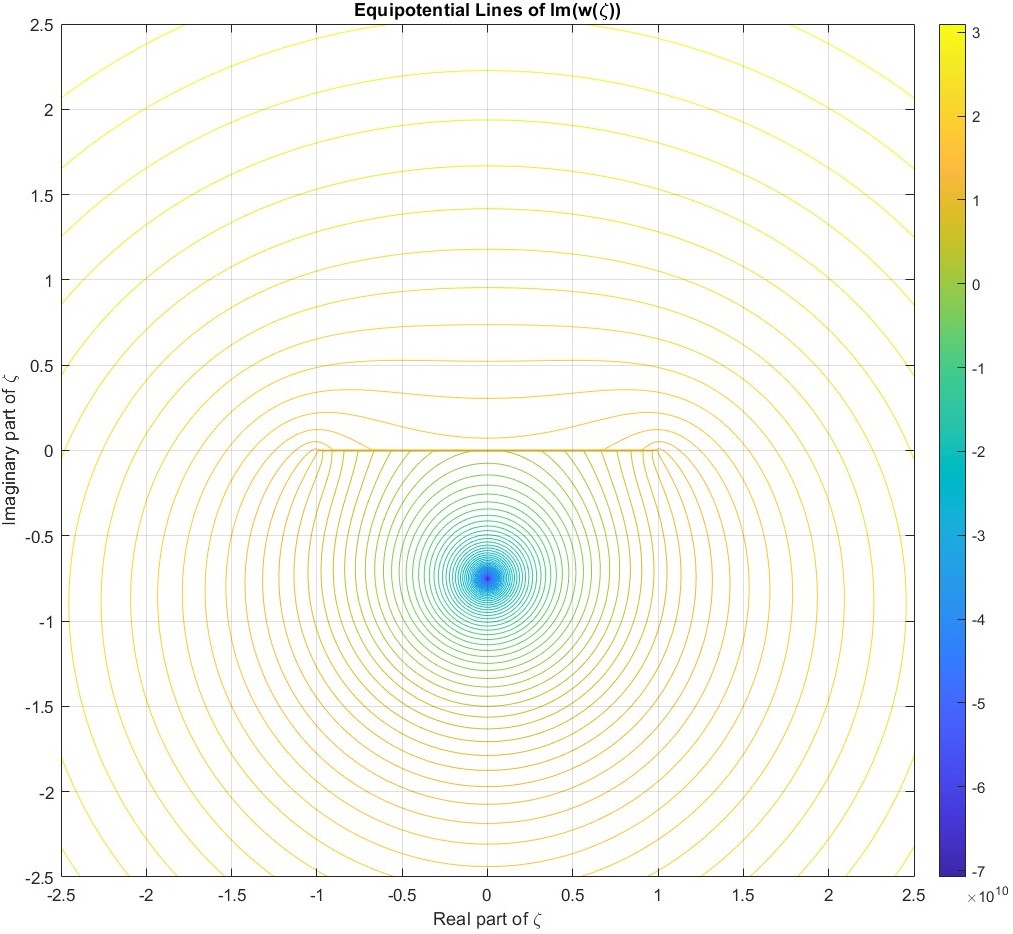
\includegraphics[width=0.75\linewidth]{Figs/slit, Pot out dielectric.jpg}
    \caption{Enter Caption}
    \label{fig:wrong pot}
\end{figure}
\pagebreak
%\renewcommand\bibname{{References}}
%\bibliography{References}
%\bibliographystyle{plain}
\chapter{Link to the Project's GitHub repository}
\hspace{0em}\noindent The relevant content will be supplemented and modified gradually

For the MATLAB and Mathematica code, please visit the GitHub repository: \url{https://github.com/Yuan-uoa/MSc_App_maths_Project/tree/main}.


\end{document}